\documentclass[spanish,unknownkeysallowed]{beamer}
%% \usetheme{Warsaw}
%% \usetheme{Madrid}

\usepackage[spanish]{babel}
\usetheme[beetle]{Boadilla}


 \useoutertheme{miniframes}
%% \useinnertheme{rounded}
%% \usecolortheme{}
\usepackage[utf8]{inputenc}
\usepackage{tikz}
\usepackage{wrapfig}
\usepackage{algorithmic, algorithm}
%% \usepackage{authblk}


%% \setbeameroption{show notes}


\usepackage{graphicx} 
%\usepackage{algorithmic}
%\usepackage{algorithm}
\newcommand{\formulasize}{\tiny}

\definecolor{rojo}{rgb}{0.7,0.1,0.1}
\definecolor{azul}{rgb}{0.1,0.1,0.7}
\definecolor{verde}{rgb}{0.1,0.4,0.1}

\newcommand{\rojo}[1]{\textcolor{rojo}{#1}}
\newcommand{\azul}[1]{\textcolor{azul}{#1}}
\newcommand{\verde}[1]{\textcolor{verde}{#1}}

%% \setcounter{secnumdepth}{5}

\newcommand{\Rojo}[1]{\textbf{\rojo{#1}}}
\newcommand{\Azul}[1]{\textbf{\azul{#1}}}
\newcommand{\Verde}[1]{\textbf{\verde{#1}}}

%%% Unified concepts commands

\newcommand{\opencl}{\emph{OpenCL}}

\newcommand{\pipeline}{\emph{pipeline}}
\newcommand{\Pipeline}{\emph{Pipeline}}

\newcommand{\wi}{\emph{work item}}
\newcommand{\wis}{\emph{work items}}
\newcommand{\wg}{\emph{work group}}
\newcommand{\wgs}{\emph{work groups}}

\newcommand{\Wi}{\emph{Work item}}
\newcommand{\Wis}{\emph{Work items}}
\newcommand{\Wg}{\emph{Work group}}
\newcommand{\Wgs}{\emph{Work groups}}

\newcommand{\bbox}{BBox}
\newcommand{\bboxes}{BBoxes}
\newcommand{\bvh}{BVH}
\newcommand{\bvhs}{BVHs}

\newcommand {\raytracer}{\emph{ray tracer}}
\newcommand {\raytracers}{\emph{ray tracers}}
\newcommand {\raytracing}{\emph{ray tracing}}
\newcommand {\Raytracer}{\emph{Ray tracer}}
\newcommand {\Raytracers}{\emph{Ray tracers}}
\newcommand {\Raytracing}{\emph{Ray tracing}}

%%% Style fix so institue doesnt appear on brackets (props to Claudio Fiandrino)
\setbeamertemplate{footline}{
  \leavevmode%
  \hbox{%
  \begin{beamercolorbox}[wd=.333333\paperwidth,ht=2.25ex,dp=1ex,center]{author in head/foot}%
    \usebeamerfont{author in head/foot}\insertshortauthor
  \end{beamercolorbox}%
  \begin{beamercolorbox}[wd=.333333\paperwidth,ht=2.25ex,dp=1ex,center]{title in head/foot}%
    \usebeamerfont{title in head/foot}\insertshorttitle
  \end{beamercolorbox}%
  \begin{beamercolorbox}[wd=.333333\paperwidth,ht=2.25ex,dp=1ex,right]{date in head/foot}%
    \usebeamerfont{date in head/foot}\insertshortdate{}\hspace*{2em}
    \insertframenumber{} / \inserttotalframenumber\hspace*{2ex} 
  \end{beamercolorbox}}%
  \vskip0pt%
}

\begin{document}
\title
    [Modelado Foto-Realístico de Materiales]{Modelado y Simulación Foto-Realística de Materiales}

\author[Lic. Rodrigo Baravalle]{Lic. Rodrigo Baravalle}
 
\institute[UNR]{
    FCEIA, Universidad Nacional de Rosario. CIFASIS-CONICET.
}

\date{Tesis Doctoral, Marzo 2016}

\begin{frame}
\begin{figure}
{
\includegraphics[width=0.08\textwidth]{../figures/logounr}}
\end{figure}
\vspace{-1cm}
  \titlepage
\centering
\vspace{-.4cm}
\begin{tiny}
Director: Dr. Claudio Delrieux, UNS

Co-Director: Dr. Juan Carlos Gómez, UNR

\ \\

\it{Miembros del jurado:}

Dr. Néstor Calvo (UNL)

Dr. Marcelo Vénere (UNICEN)

Dr. Gustavo Galizzi (UNR)

\end{tiny}

\end{frame}
%%%%%%%%%%%%%%%%%%%%%%%%%%%

\section{Introducción}

\begin{frame}
\begin{block}{}
\begin{center}
\vspace{1cm}
\huge{Introducción}
\vspace{1cm}
\end{center}
\end{block}
\end{frame}


\subsection{Modelado y Simulación Foto-Realística}
\begin{frame}{Modelado foto-realístico de escenas}



\centerline{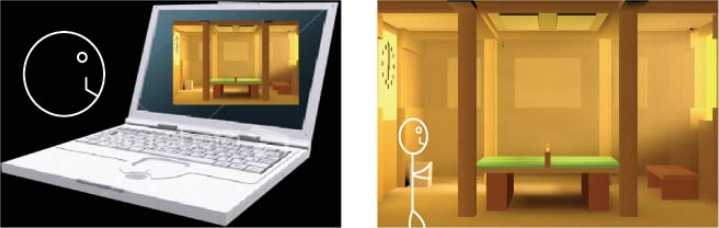
\includegraphics[scale = 0.25]{../figures/fotorealismo}}

\textbf{Foto-realismo}: síntesis de imágenes que produzcan el \textbf{mismo efecto}, en la percepción, que una fotografía del material/escena.

\vspace{0.2cm}

El área experimentó avances notables desde su concepción.
\begin{block}{}
\begin{itemize}
\item \textbf{Nivel de Realismo}: se desarrollaron teorías computacionales que modelan fenómenos físicos subyacentes ({\it e.g.} Ecuación del Renderizado de Superficies y Volúmenes).
\item \textbf{Velocidad}: tasas de tiempo interactivo / real: evolución cuasi-exponencial del poder de cómputo (GPU's).
\end{itemize}
\end{block}

\end{frame}

\begin{frame}

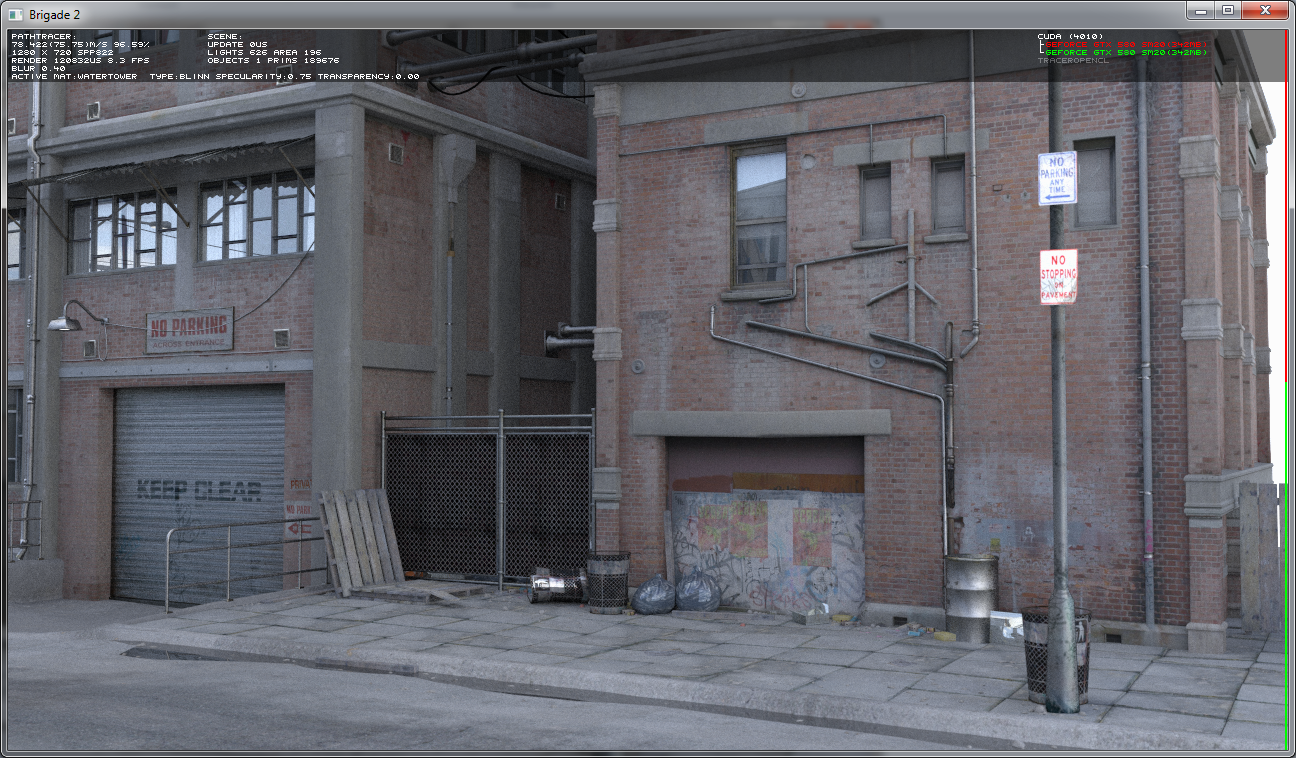
\includegraphics[scale = 0.18]{../figures/hd1.png}
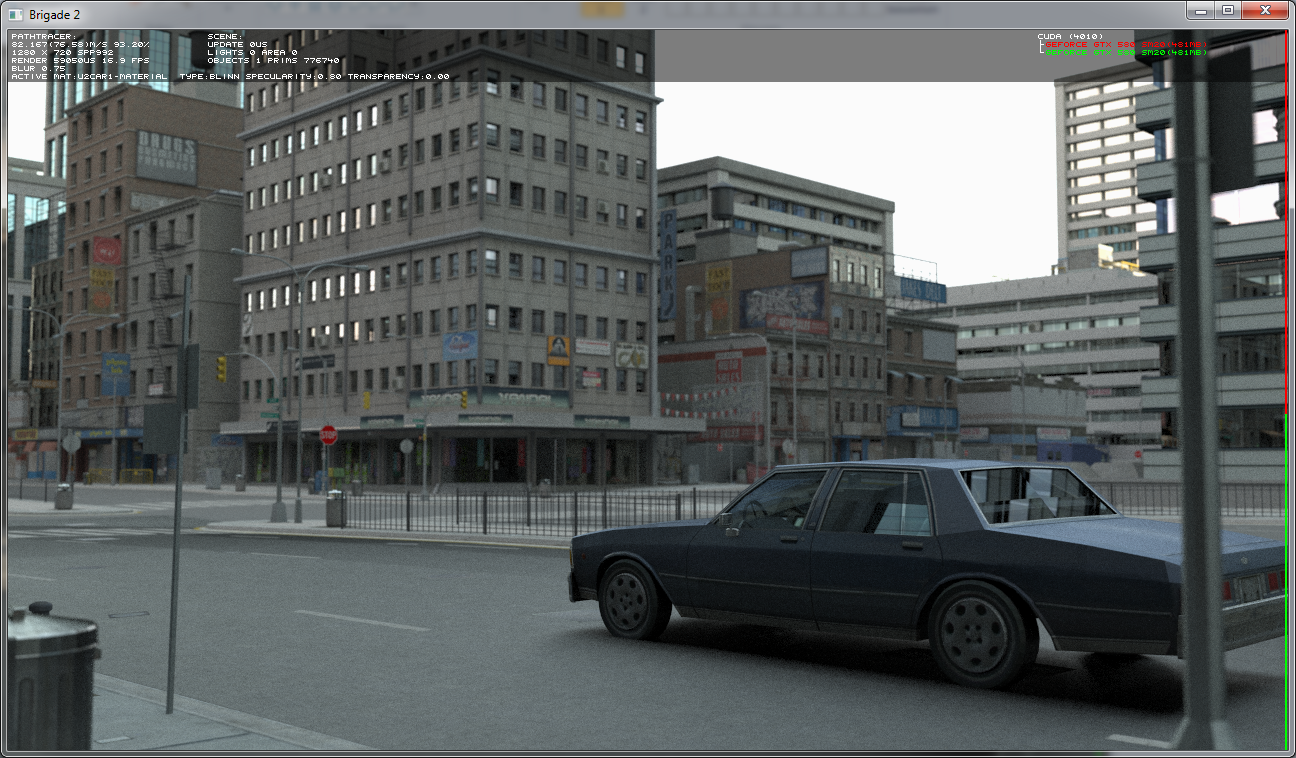
\includegraphics[scale = 0.18]{../figures/blinn5ed.png}

(Imágenes: Brigade 2 Renderer)


\end{frame}




\begin{frame}{Síntesis de la Imagen de una Escena}
\textbf{Renderización}:
Computar \textbf{radiancia} que arriba a la \textbf{cámara} desde toda la escena.

\vspace{0.4cm}
La radiancia \textit{entrante}, a cada píxel, depende de numerosos factores
\begin{itemize}
\item \textbf{forma} del objeto
\item \textbf{material}, 
\item \textbf{oclusión} existente entre el objeto y la cámara
\item temperatura
\item etc.
\end{itemize}


\vspace{0.4cm}
Cada objeto de la escena puede emitir radiancia (en todo el espectro electromagnético) hacia el observador.

\end{frame}



\begin{frame}[Luz]
\begin{block}{Luz}
\begin{itemize}
\item La comprensión del fenómeno evolucionó considerablemente a lo largo del tiempo.
%\item ``dualidad onda-partícula'': Debe simplificarse su tratamiento en computación gráfica.
\item En la mayoría de los casos, sólo la \textbf{luz visible} es la que debe modelarse (apariencia).
\item Se asume distribución en líneas rectas o \textbf{rayos} (representación {\em óptico geométrica}, escala macroscópica).
\end{itemize}
\end{block}

\begin{block}{Debe modelarse, además, su interacción con \textbf{cada objeto}}
Modelado de la \textbf{geometría}.
\end{block}

\end{frame}


\begin{frame}{Materiales}
\textbf{Apariencia} de un material
\begin{itemize}
\item Definición informal: {\em percepción} del mismo por parte de una persona.
\item Conjunto de estímulos visuales.
\end{itemize}

Depende de la escala buscada
\begin{itemize}
\item \textbf{Microscópico}: detalles invisibles al ojo humano (técnicas estadísticas)
\item \textbf{Macroscópico}: visible (triángulos, texturas, etc)
\end{itemize}

Estudio del material $\rightarrow$ comprensión de su apariencia $\rightarrow$ modelo numérico

\centerline{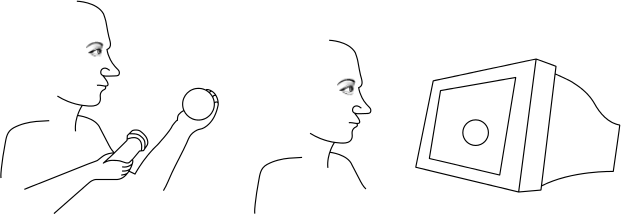
\includegraphics[scale = 0.25]{../figures/apariencia}}
\end{frame}


\begin{frame}{}

\begin{block}{Materiales con mayor aparición en escenas}

Agua, Piel humana, Metales, Plásticos, etc. 

Posibles causas: \textbf{facilidad} del diseño (realismo), aparición \textbf{constante} en escenas

\end{block}

\begin{block}{Materiales con menor aparición en escenas}
Materiales cocidos, porosos y comestibles


\begin{itemize}
\item \textbf{Geometría compleja y visible}
\item \textbf{Fácil detección} de modelos inadecuados
\item \textbf{Costo computacional} excesivo
\end{itemize}
\end{block}

{\it Alain Fournier: `computer graphics has still not been
able to convincingly render a slice of bread' (2001)}


\end{frame}

\begin{frame}
\begin{block}{}
Debido a las consideraciones anteriores, en esta tesis haremos hincapié en materiales \textbf{porosos}.

Objetivos
\begin{itemize}
\item Producir una geometría configurable, intuitiva y creíble de estos materiales.
\item Implementación de un modelo inspirado en procesos físicos en la formación de un material poroso: el pan.
\item Se busca \textbf{renderización foto-realista} en tiempo interactivo/real.
\item Se busca \textbf{validar} los resultados.
\end{itemize}

%La tesis presenta algunos resultados favorables inesperados
%\begin{itemize}
%\item Caracterización y clasificación de imágenes de pan
%\item Generación de texturas de materiales no porosos (madera, mármol..)
%\end{itemize}


\end{block}
\end{frame}


\subsection{Trabajo Previo}

\begin{frame}{Modelado de la Geometría}

\textbf{Problema}

Supervisión humana repetitiva. Ejemplo: diseñar separadamente cada árbol de un bosque

\begin{block}{Solución}
Técnicas \textbf{Procedimentales} (técnicas semi-automáticas basadas en algoritmos)
\end{block}

\begin{block}{Sistemas-L (Lindenmayer)}

Describen la estructura visible de plantas


\begin{itemize}
\item \textbf{axioma}, reglas \textbf{reglas de producción}, número de iteraciones
\end{itemize}
\end{block}

%En cada iteración se aplican reglas de producción a la cadena de caracteres resultante anterior.

Axioma: $F$, $P1: F \rightarrow FfF$.

$F \rightarrow FfF \rightarrow \textbf{FfF}f\textbf{FfF} \ldots$

\end{frame}

\begin{frame}{Ejemplo}
\begin{itemize}
\item Estado inicial ($x$,$y$,$90^{\circ}$)
\item \textbf{Axioma:} F
\item Regla de producción $F \rightarrow FF-FfF-FF$
\end{itemize}

%\begin{itemize}
%\item F, moverse hacia adelante un paso $d$, dibujando,
%\item f, moverse hacia adelante un paso $d$, sin dibujar,
%\item +, rotar un ángulo $\delta$,
%\item -, rotar un ángulo $-\delta$.
%\end{itemize}

\center
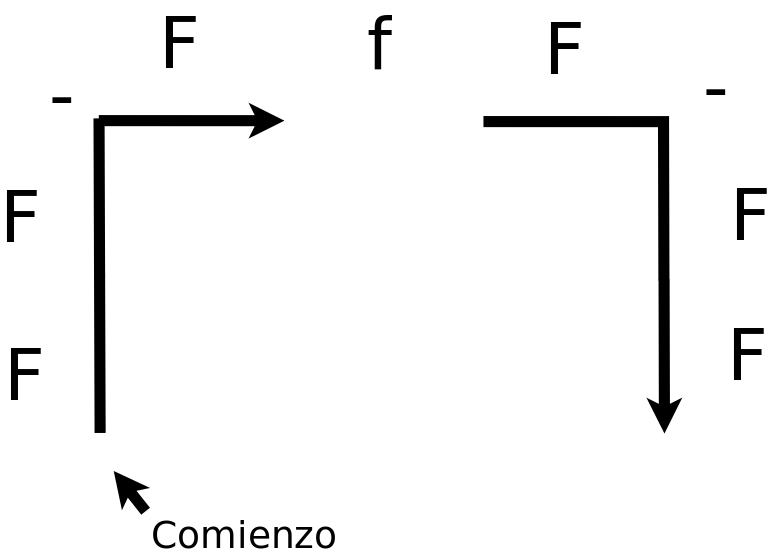
\includegraphics[width=4cm]{../figures/tortuga}

\end{frame}

\begin{frame}{Sistemas-L: Arboles}
Pila de estados
\begin{itemize}
\item $[$ : estado actual $\rightarrow$ pila ({\em push})
\item $]$ : cabeza de la pila $\rightarrow$ estado actual ({\em pop}):
\end{itemize}

\center
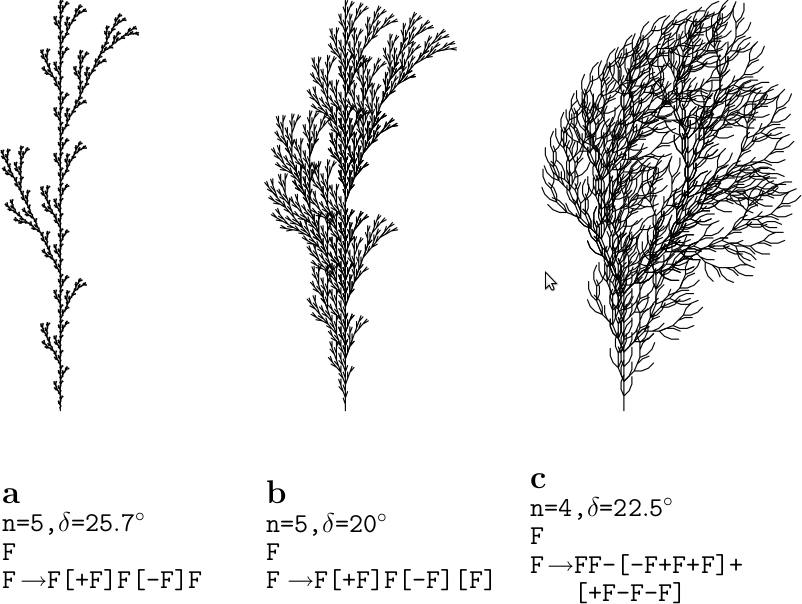
\includegraphics[width=6.3cm]{../figures/sistemalcorchete}
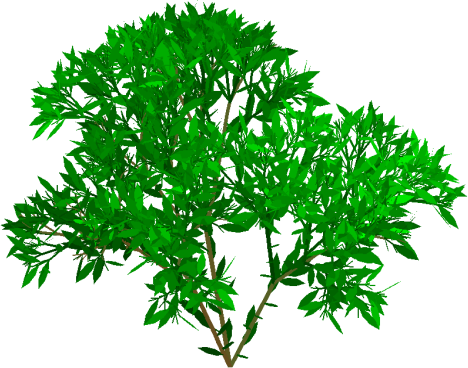
\includegraphics[width=5cm]{../figures/3dlsystem}

\end{frame}

\begin{frame}{}
\begin{block}{Sistemas-L}
\textbf{Comparación subjetiva}: objeto sintético $\leftrightarrow$ objeto real
\end{block}

\begin{block}{Modelado Físico de materiales}

Ecuaciones del \textbf{comportamiento} o \textbf{crecimiento} de los mismos.

\textbf{Ecuaciones de Navier-Stokes} (fluídos)
\center
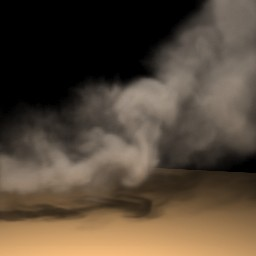
\includegraphics[width=3cm]{../figures/smoke}
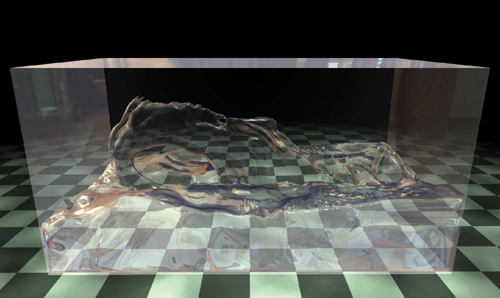
\includegraphics[width=6cm]{../figures/water}
\end{block}

%Dadas condiciones iniciales $\bold{u}$ y $p$ cuando $t = 0$,
%\begin{align*}
%\nabla \cdot \bold{u} &= 0\\
%\frac{\partial \bold{u} }{\partial t} &= - (\bold{u} \cdot \nabla) \bold{u} - \frac{1}{\rho} \nabla p + \nu \nabla^{2} \bold{u} + \bold{f},
%\end{align*}

%\noindent donde $\nu$ representa la viscosidad cinemática del fluido, $\rho$ la densidad y $\bold{f}$ una fuerza externa.

%\end{frame}

%\begin{frame}{Ecuaciones de Navier-Stokes, humo}


\end{frame}

\subsection{Renderizado}

\begin{frame}
Las geometrías obtenidas deben \textbf{renderizarse} para ser visualizadas.
\vspace{0.5cm}

Se desarrollaron ecuaciones que representan el comportamiento de la luz en una escena.
Las mismas obtienen imágenes \textbf{foto-realistas} de escenas y materiales.

Existen dos clases principales de técnicas de modelado:

\begin{block}{}
\begin{itemize}
\item Superficies (Metales, plásticos)
\item Volúmenes (Humo, fuego)
\end{itemize}
\end{block}
\end{frame}


\begin{frame}{Ecuación del Renderizado de Superficies:}

\textbf{Radiancia entrante} en $x$ (por medio de \textbf{todos} los puntos $x'$ de \textbf{todas las superficies}).

\centerline{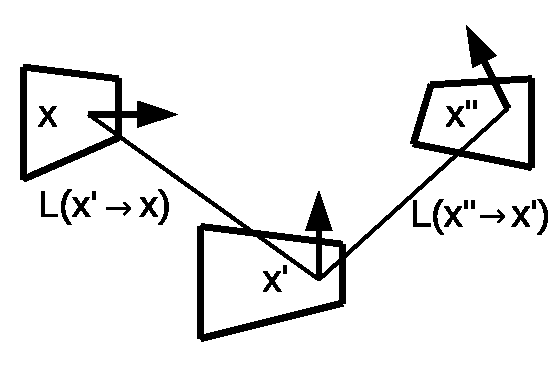
\includegraphics[scale = 0.4]{../figures/rendequation}}
\vspace{-1cm}
$$ L(\bold{x'} \rightarrow \bold{x}) =  g(\bold{x'}  \rightarrow \bold{x})  \left[ \epsilon(\bold{x'}  \rightarrow \bold{x}) + \int_{s}{\rho(\bold{x''}  \rightarrow \bold{x'}  \rightarrow \bold{x})L(\bold{x''}  \rightarrow \bold{x}) d\bold{x''}} \right] $$

\textbf{Recursiva}
%: la \textbf{energía radiante saliente} de $x'$ depende de la \textbf{energía radiante entrante} desde todos los puntos de todas las superficies.

$\bold{x}$,$\bold{x'}$ y $\bold{x''}$ varían sobre todas las superficies.

(Ray Tracing, Path Tracing)

\end{frame}

%\begin{frame}
%$$ L(\bold{x'} \rightarrow \bold{x}) =  g(\bold{x'}  \rightarrow \bold{x})  \left[ \epsilon(\bold{x'}  \rightarrow \bold{x}) + \int_{s}{\rho(\bold{x''}  \rightarrow \bold{x'}  \rightarrow \bold{x})L(\bold{x''}  \rightarrow \bold{x}) d\bold{x''}} \right] $$

%\begin{itemize}
%\item $L(\bold{x'} \rightarrow \bold{x})$, intensidad de la luz que viaja del punto tridimensional $\bold{x'}$ a $\bold{x}$
%(sin oclusiones)

%\item $g(\bold{x'} \rightarrow \bold{x})$: término geométrico que modela la oclusión que podría existir entre $\bold{x}$ y $\bold{x'}$,
%\item $\epsilon(\bold{x'} \rightarrow \bold{x})$ intensidad de la luz emitida desde $\bold{x'}$ a $\bold{x}$,
%\item $\rho(\bold{x''}  \rightarrow \bold{x'}  \rightarrow \bold{x})$ la intensidad de la luz emitida de $\bold{x''}$ a $\bold{x}$ por medio de una superficie en $\bold{x'}$ (esta cantidad será llamada función bidireccional de distribución de reflectancia, BRDF),

%\item $S=\bigcup{s_{i}}$, unión de todas las superficies $s_{i}$ de la escena
%\end{itemize}
%\end{frame}

%\begin{frame}

%\begin{equation*}
%L(\bold{x'} \rightarrow \bold{x}) =  g(\bold{x'}  \rightarrow \bold{x})  \left[ \epsilon(\bold{x'}  \rightarrow \bold{x}) + \int_{s}{\rho(\bold{x''}  \rightarrow \bold{x'}  \rightarrow \bold{x})L(\bold{x''}  \rightarrow \bold{x}) d\bold{x''}} \right]
%\end{equation*}


%Además se asume una superficie $S_{0}$, la cual se modela como una semi-esfera que engloba a toda la escena.

%\vspace{0.2cm}
%Aproximación de las propiedades óptico-geométricas de las ecuaciones del electromagnetismo de Maxwell.

%(Ray Tracing, Path Tracing)
%\end{frame}


\begin{frame}{Ecuación del Renderizado de Volúmenes}
Cambio de radiancia ($L$) en una dirección dada ($\vec{\omega}$) 

Absorción, dispersión saliente, emisión y dispersión entrante.
\begin{equation*}
\begin{aligned}
(\vec{\omega} \cdot \nabla) L(\bold{x} \rightarrow \vec{\omega}) = - \sigma_{a}(\bold{x}) L(\bold{x} \rightarrow \vec{\omega}) - \sigma_{s}(\bold{x}) L(\bold{x} \rightarrow \vec{\omega}) + \\
\sigma_{a}(\bold{x}) L_{e}(\bold{x} \rightarrow \vec{\omega}) + \sigma_{s}(\bold{x}) L_{i}(\bold{x} \rightarrow \vec{\omega}).
\end{aligned}
\end{equation*}

$\sigma_{a}$: coef. absorción, $\sigma_{s}$: coef. dispersión.

%\end{frame}

%\begin{frame}{Ecuación del Renderizado de Volúmenes}
\centering
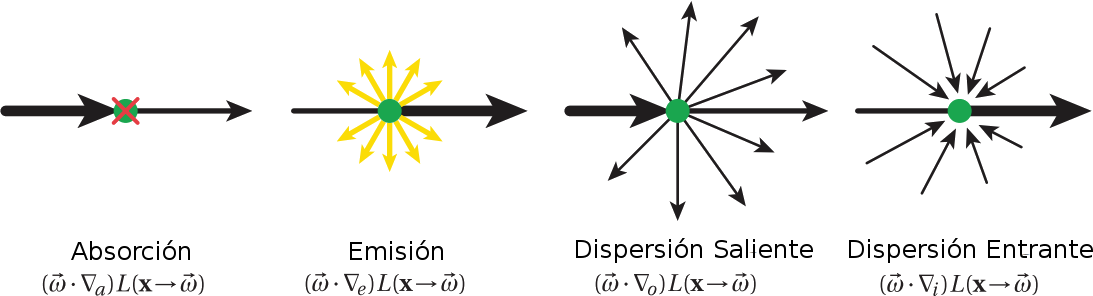
\includegraphics[scale = 0.3]{../figures/fenomenosrte}

Ray Casting (Direct Volume Rendering)
\end{frame}



\subsection{Materiales porosos}


\begin{frame}{Materiales porosos - Trabajo Previo}

Volúmenes
\begin{block}{}
\begin{itemize}
\item \textbf{cortes arbitrarios} en el objeto
\item \textbf{más costosos}, (almacenamiento, tiempo de renderizado)
\end{itemize}
\end{block}

Se utilizan diversos ruidos

\begin{itemize}
\item Voronoi, Perlin, Worley. $+$ consideraciones ad-hoc
\end{itemize}

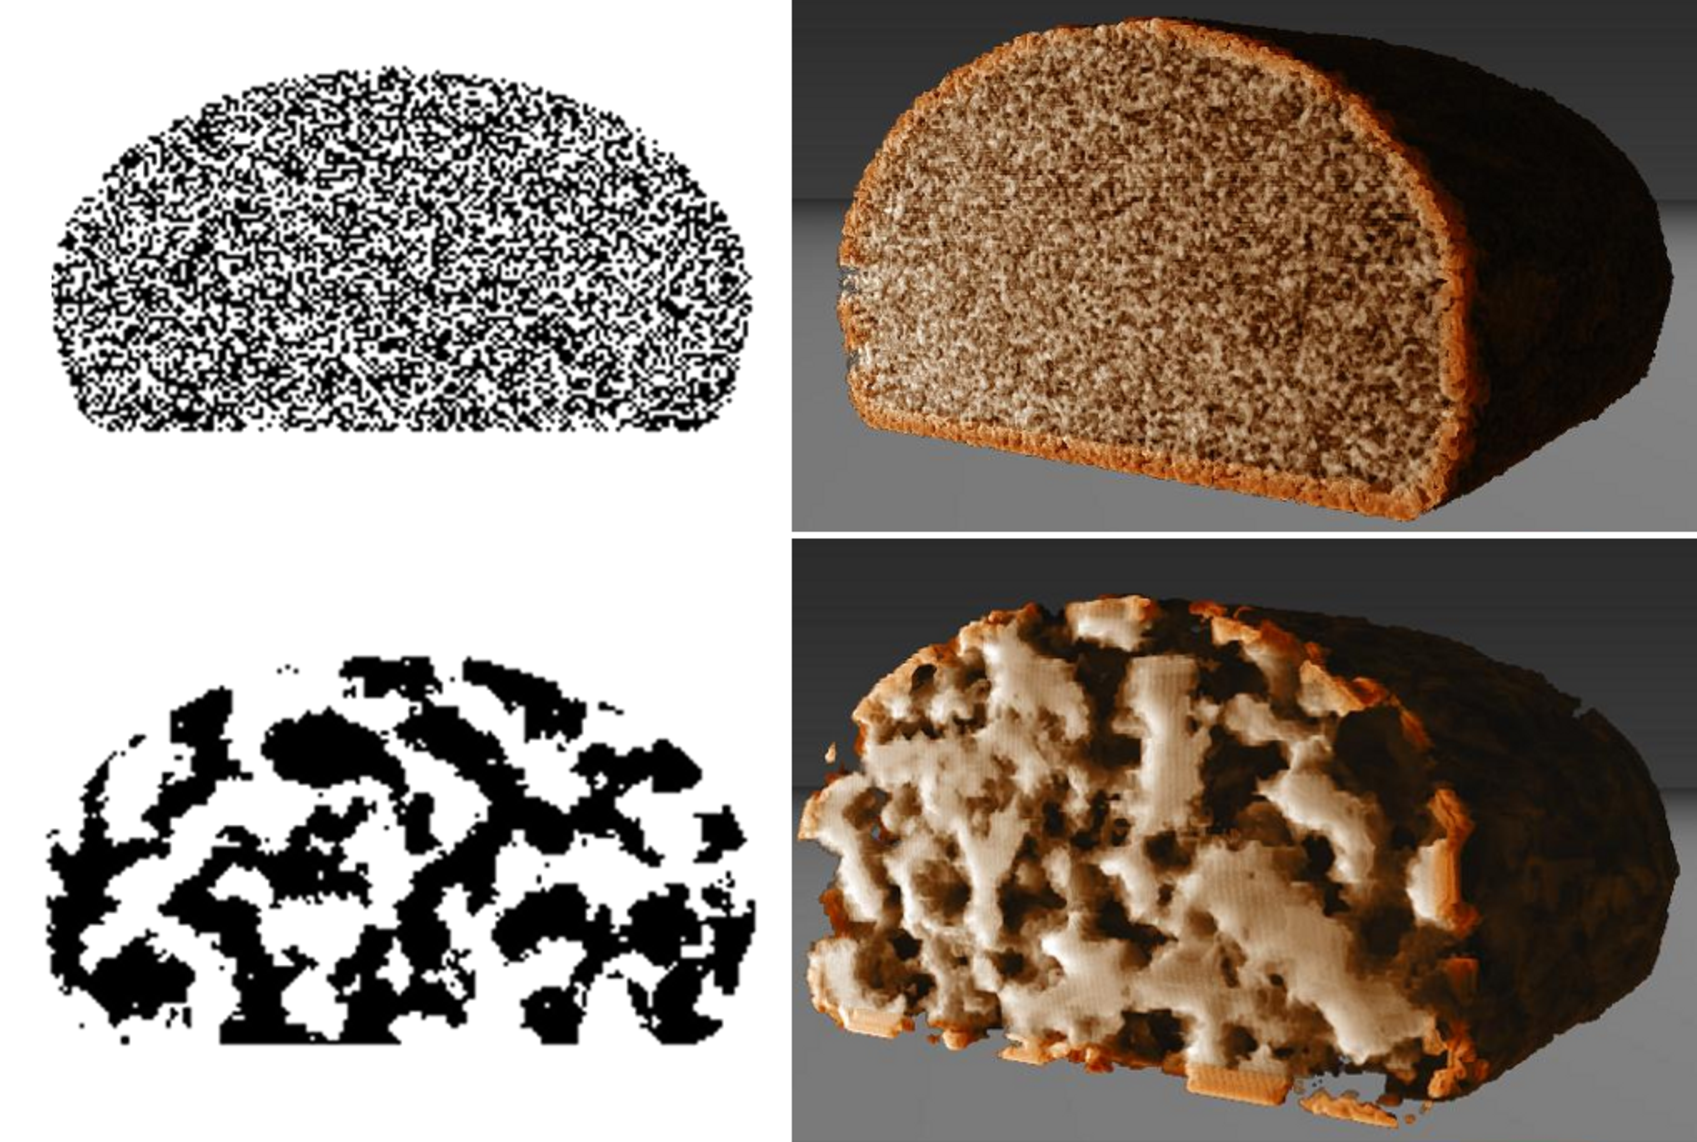
\includegraphics[scale = 0.15]{../figures/Fig8}
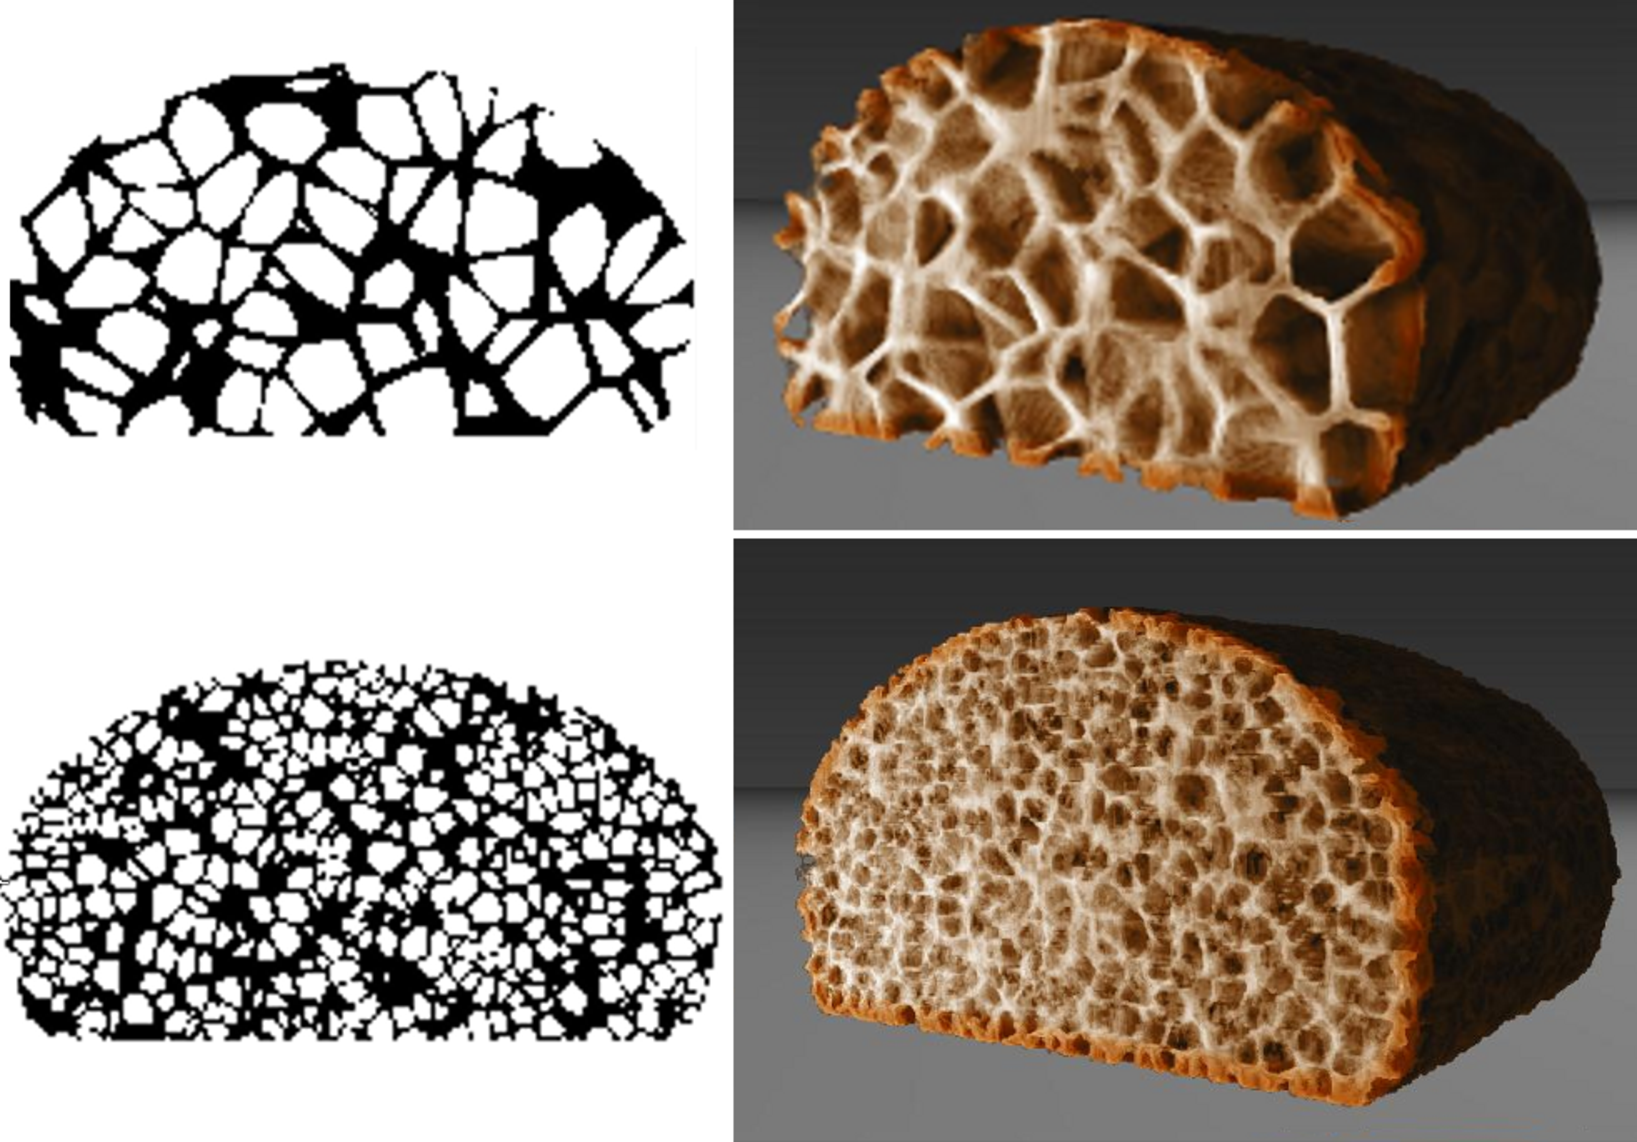
\includegraphics[scale = 0.15]{../figures/Fig9CAVW}
\end{frame}


\begin{frame}{Materiales porosos - Trabajo Previo}
Desventajas: 
\begin{block}{}
\begin{itemize}
\item control sobre cantidad y tamaño de las burbujas
\item deformación de burbujas
\item el usuario debe ser experto
\end{itemize}
\end{block}

Ratatouille (Película): Voronoi + mapa (deformación de burbujas).
\centering{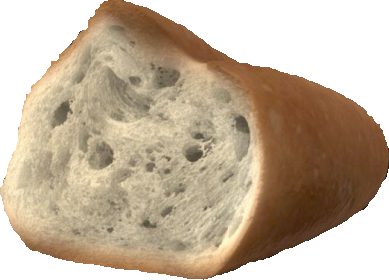
\includegraphics[scale = 0.3]{../figures/ratatouille}}

\end{frame}

\begin{frame}

Superficies: {\it Tong et al (2005)}

Capturas (cámaras y lásers) $\rightarrow$ distribuciones precisas de radiancia.

\begin{itemize}
\item Proceso de captura muy complejo
\item Limitado a una geometría
\item Tiempos de cómputo?
\item Imposibilidad de realizar cortes
\end{itemize}

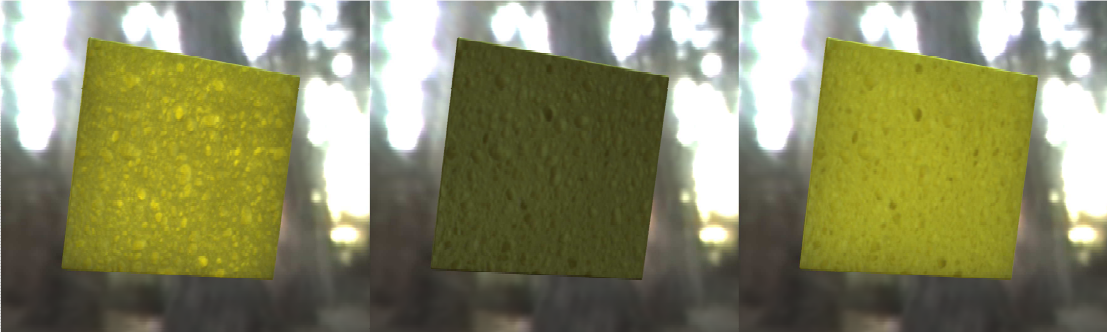
\includegraphics[scale = 0.3]{../figures/esponja}

\end{frame}


\section[Mod. de Materiales Porosos]{Modelado Procedimental de Materiales Porosos}

\begin{frame}
\begin{block}{}
\begin{center}
\vspace{1cm}
\huge{Modelado Procedimental de Materiales Porosos}
\vspace{1cm}
\end{center}
\end{block}
\end{frame}

\subsection{Modelado Procedimental de Materiales Porosos}
\begin{frame}{Modelado de Geometrías Porosas - Propuesta}
Presentamos un modelo de generación de geometrías porosas basados en:
\begin{itemize}
\item \textbf{Sistemas de Partículas} que crecen, evitándose
\item \textbf{Sistemas dinámicos} como medio de crecimiento
\end{itemize}

\vspace{0.4cm}

\textbf{Sistemas de partículas}
\begin{itemize}
\item Partícula: posición, dirección, color, tiempo de vida, etc.
\item Fluídos, objetos con interfaces sin definición precisa

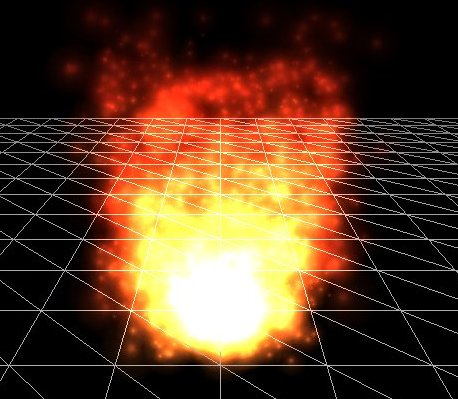
\includegraphics[scale = 0.216]{../figures/fire}
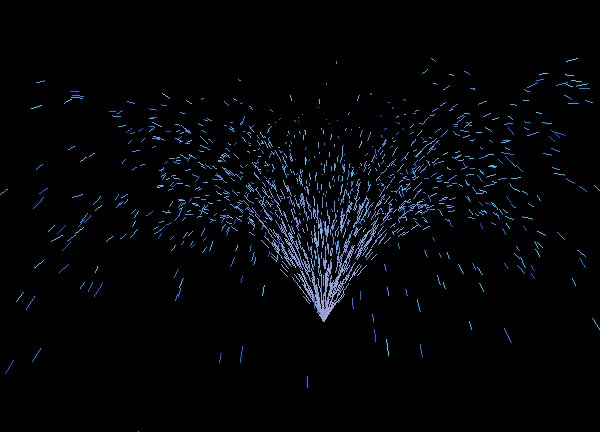
\includegraphics[scale = 0.2]{../figures/fireworks}
\end{itemize}
\end{frame}

\begin{frame}
El sistema consta de:
\begin{itemize}
\item un conjunto de partículas $P = \{p_{1}, ... , p_{n}\}, n  \in \mathbb{N}$
\item y dos grillas, $L_{N\times N \times N},$, $L^{2}_{N\times N \times N}, N \in \mathbb{N}.$
\end{itemize}

%Condiciones Iniciales:
%\begin{itemize}
%\item $L_{xyz}=1$: masa
%\item $L^{2}_{xyz}=-1$: celda libre,
%\end{itemize}

Cada partícula posee:
\begin{equation*}
  p_{i} = \{O_{i}, C_{i}\}, 1 \le i \le n,
\end{equation*}

\begin{itemize}
\item $O_{i} = \{o_{1}, ... , o_{n_{i}}\}$:posiciones ocupadas por la part\'icula en $L$.

\item $C_{i} = \{c_{1}, ... , c_{m_{i}}\}$:posiciones en el {\em contorno} de la part\'icula en $L$.
\end{itemize}

\end{frame}

%\begin{frame}

%\begin{algorithm}[H]
%\begin{algorithmic}[1]
%        \IF {$vacio?~C[i]$}
%            \STATE{morir()}
%        \ENDIF
%        \FOR{$h \in C[i]$}
%            \STATE{$C[i].eliminar(h)$}
%            %\COMMENT{la posición ya fue explorada}
%            %\STATE{// Si la pos. o contorno pertenecen a otra partícula, descartar}
%            %\STATE{// borde\_libre chequea disponibilidad en el vecindario}
%            \IF{$!(L^{2}[h] > 0 ~\&\&~ L^{2}[h] != i) ~\&\&~ borde\_libre(h,separacion)$}
%                %\State{// Posición libre, ocupar}                
%                \STATE{$L[h] \gets 0$} %\COMMENT{masa -> aire}
%                \STATE{$O[i].agregar(h)$}
%                \STATE{$C[i].agregar(vecindario(h))$} 
%                \STATE{$L^{2}.setear(vecindario(h),i)$} %\COMMENT{Marcar posiciones en $L^{2}$ como $i$}
%                \STATE{$L^{2}.setear(h,i)$}
%                \STATE{Break}
%                %\Comment{turno de la partícula $i+1$...}
%            \ENDIF
%        \ENDFOR
%\end{algorithmic}
%\label{alg:seq}
%\end{algorithm}
%\end{frame}

\begin{frame}
La partícula 14 marcó en su contorno celdas previamente marcadas por la partícula 7 en su contorno
\centerline{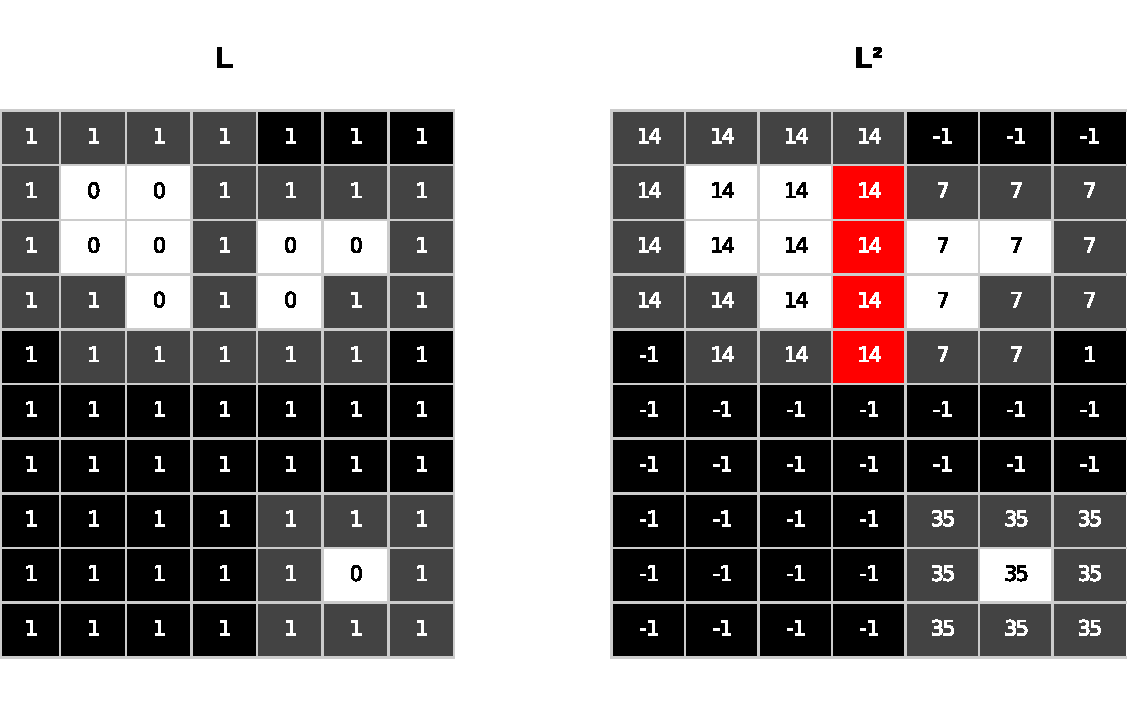
\includegraphics[scale = 0.45]{../figures/sistemaparticulas}}
La partícula 14 \textbf{no} tomará las posiciones en rojo, ya que \textbf{borde\_libre} chequea que su contorno no pertenezca a otra partícula
\end{frame}

\begin{frame}{Ejemplo: crecimiento}
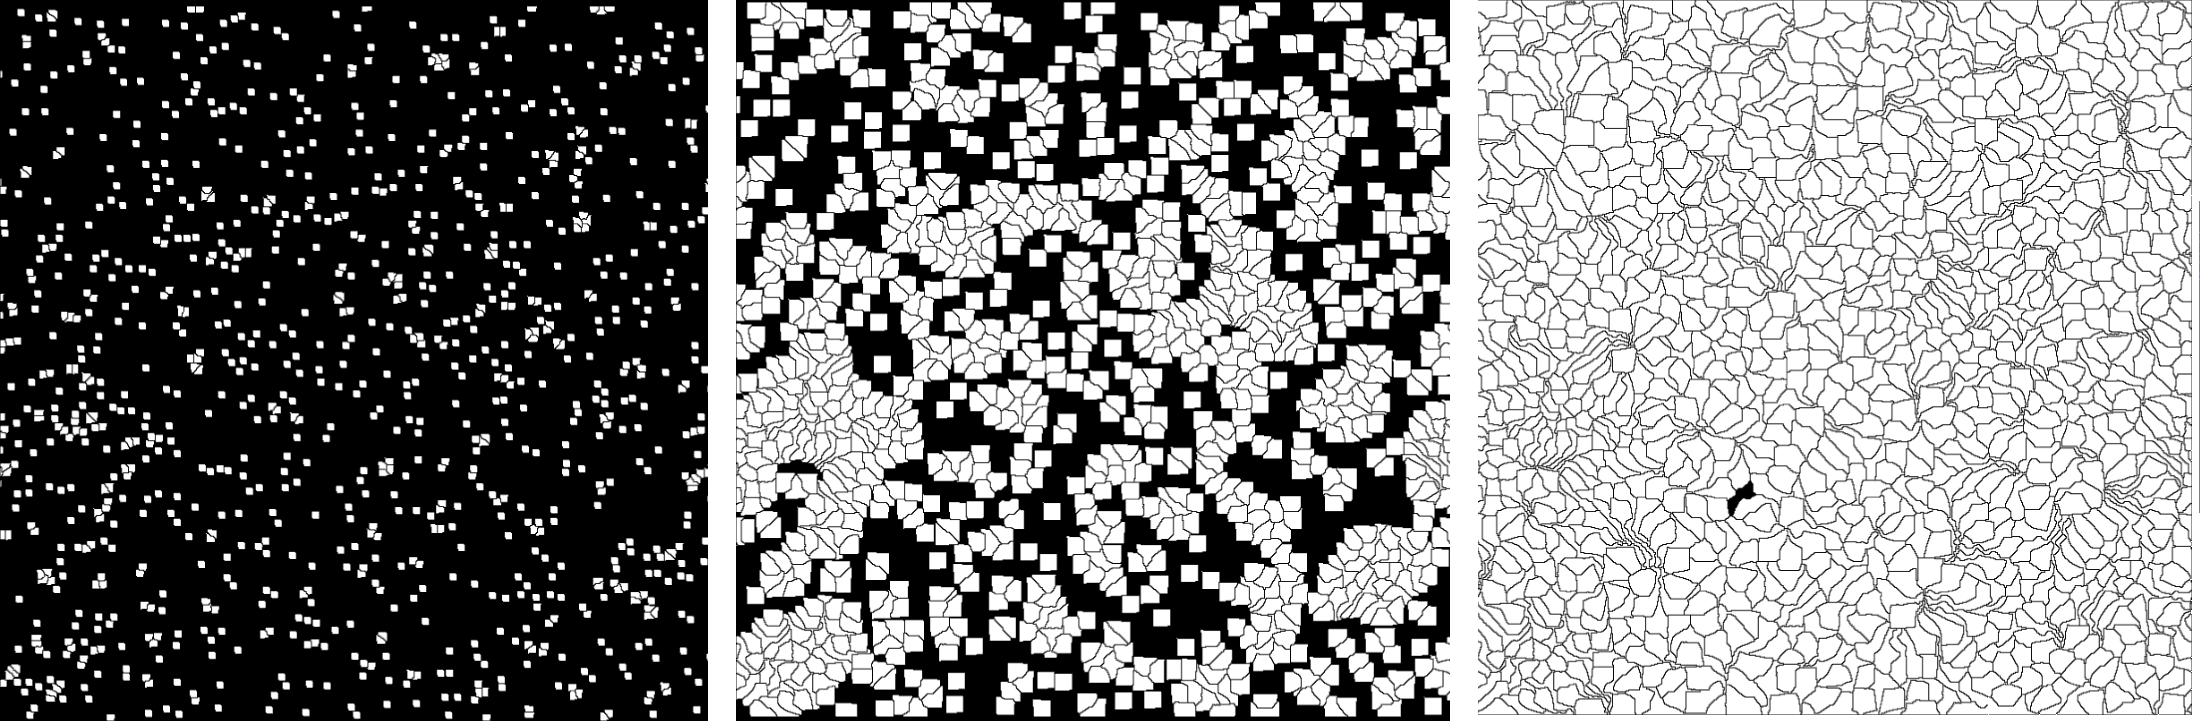
\includegraphics[scale = 0.15]{../figures/modeladocrec}

\centering
Dirección de crecimiento?
\end{frame}


\begin{frame}{Sistemas dinámicos}

Las ODEs se representan utilizando el siguiente sistema de ecuaciones:
\begin{equation*}
  \begin{aligned}
    \dot{x_{1}} = f_{1}(x_{1},\ldots,x_{n}),\\
    \ldots\\
    \dot{x_{n}} = f_{n}(x_{1},\ldots,x_{n}).
  \end{aligned}
\end{equation*}



%\end{frame}


%\begin{frame}{Crecimiento}
%Crecimiento:
%\begin{itemize}
%\item Aleatorio
%\item Direccionado
%\end{itemize}

\vspace{0.1cm}

Sistema Dinámico (SD) $\rightarrow$ campo vectorial (discreto) $\rightarrow$ dirección

%\vspace{0.1cm}

%\end{frame}

%\begin{frame}{Crecimiento}
%SD 2D, imagen izquierda:
%\begin{equation*} \label{eq:simple}  
%  \begin{aligned}
%    \dot{x} &= x^{2}-y^{2}+1,\\
%    \dot{y} &= 2xy+1.
%  \end{aligned}
%\end{equation*}
  \centerline{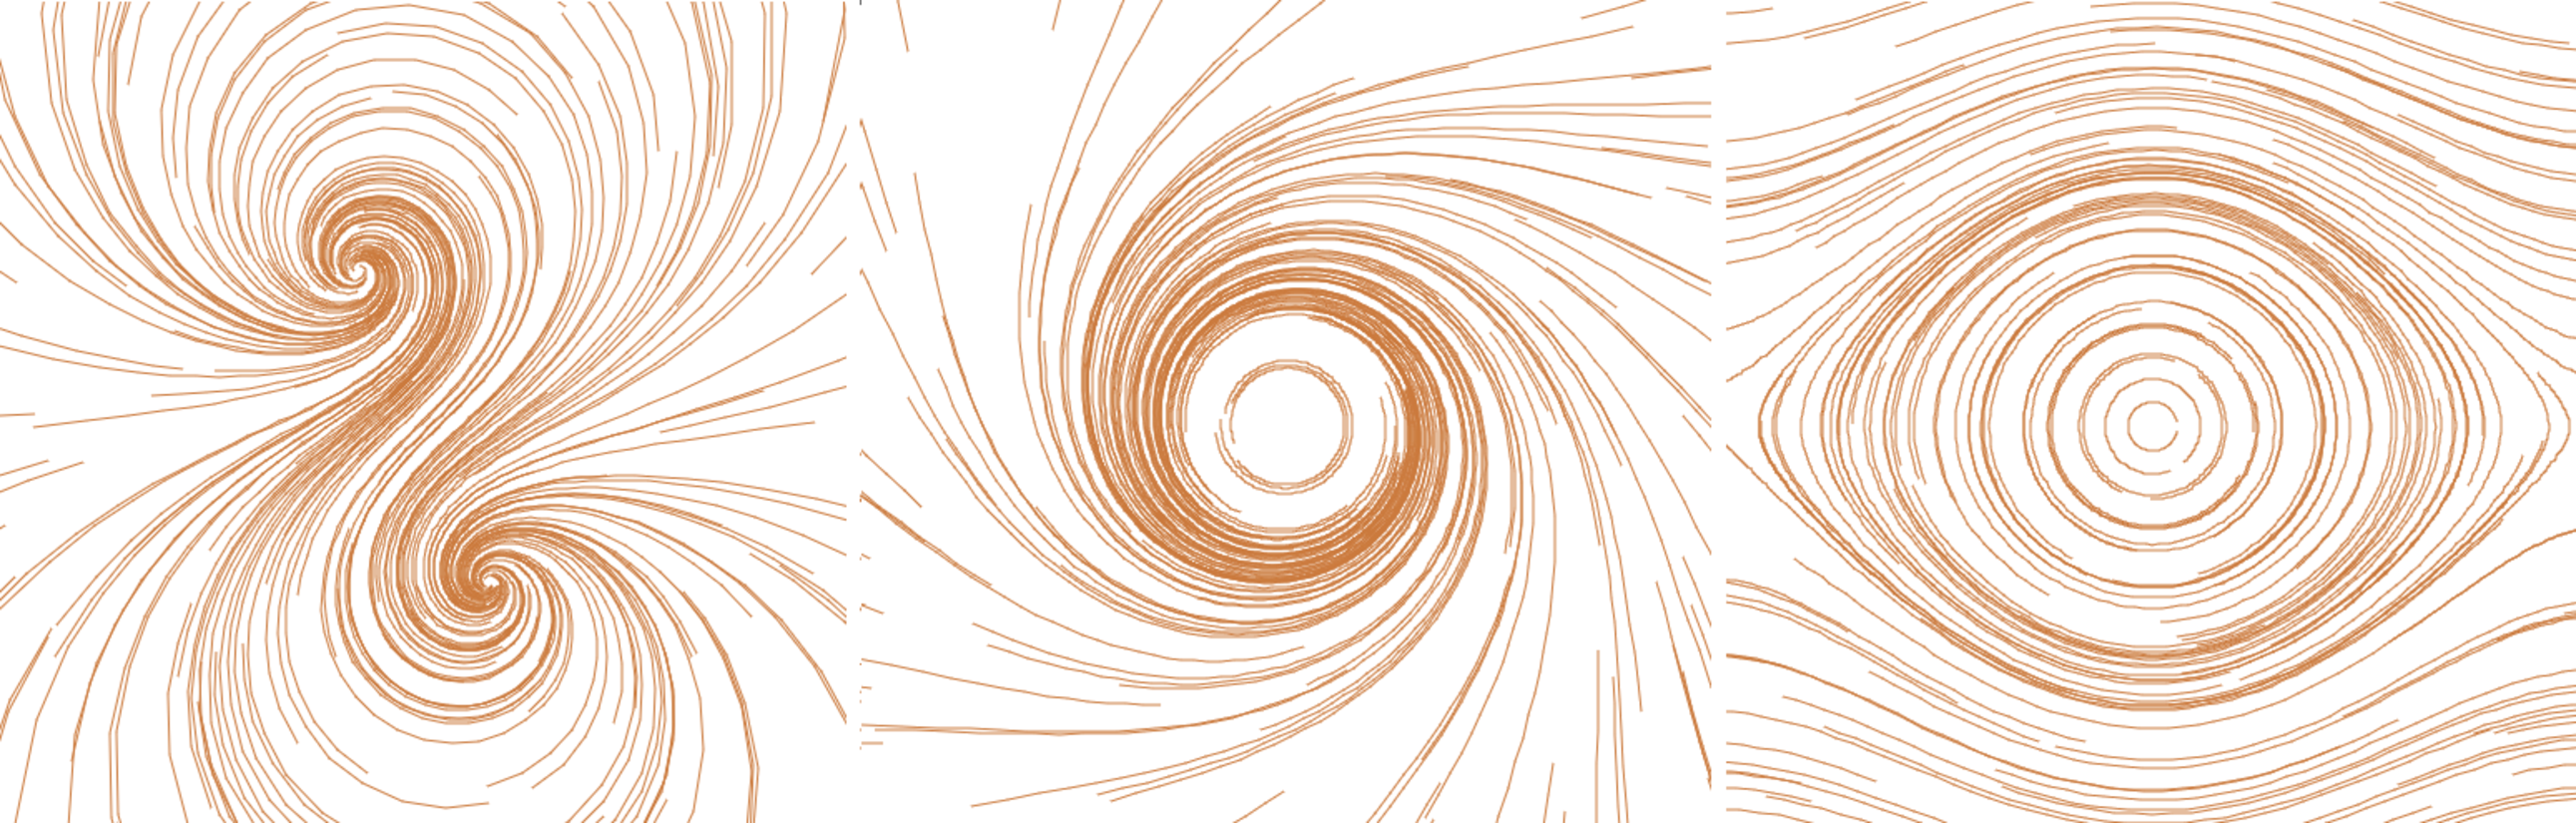
\includegraphics[width=8cm]{../figures/Fig2}}
%\end{frame}

%\begin{frame}
%Se establece una correspondencia entre los límites del plano y las posiciones de la grilla.

%\begin{itemize}
%\item Posición $(0,0)$ de la grilla $\rightarrow$ mínimo en $X$ e $Y$ (sistema dinámico)
%\item Posición $(N,N)$ con el máximo $X$ e $Y$.
%\end{itemize}

\end{frame}

%\begin{frame}
%\begin{algorithm}[H]
%\begin{algorithmic}[1]
%\STATE $solucion = Runge\_Kutta(h)$
%\STATE $vec = vecindario(h)$
%\STATE $mejor = abs(vec[0] - solucion)$
%\STATE $elegida = h$
%\STATE $vec.eliminar(h)$
%\FOR {$w \in vec$}
%%\STATE{// Se calcula la posición del vecindario que mejor aproxima al sistema}
%    \IF {$abs(vec[w]-solucion) < mejor$}
%        \STATE $mejor = abs(vec[w]-solucion)$
%        \STATE $elegida = w$
%    \ENDIF
%    \IF {$aleatorio() < aleatoriedad$} 
%    %\Comment {$0 <= aleatorio() <= 1$}
%        \STATE $C[i].agregar(w)$
%    \ENDIF
%\ENDFOR
%%\State{// Se agrega al vecindario sólo la posición que mejor aproxima la solución}
%\STATE $C[i].agregar(elegida)$
%\end{algorithmic}
%\end{algorithm}
%\end{frame}

\begin{frame}{Sistemas de partículas + Sistemas Dinámicos}

Aleatoriedad = 0.3, 0.2, y 0.1
\vspace{0.1cm}
  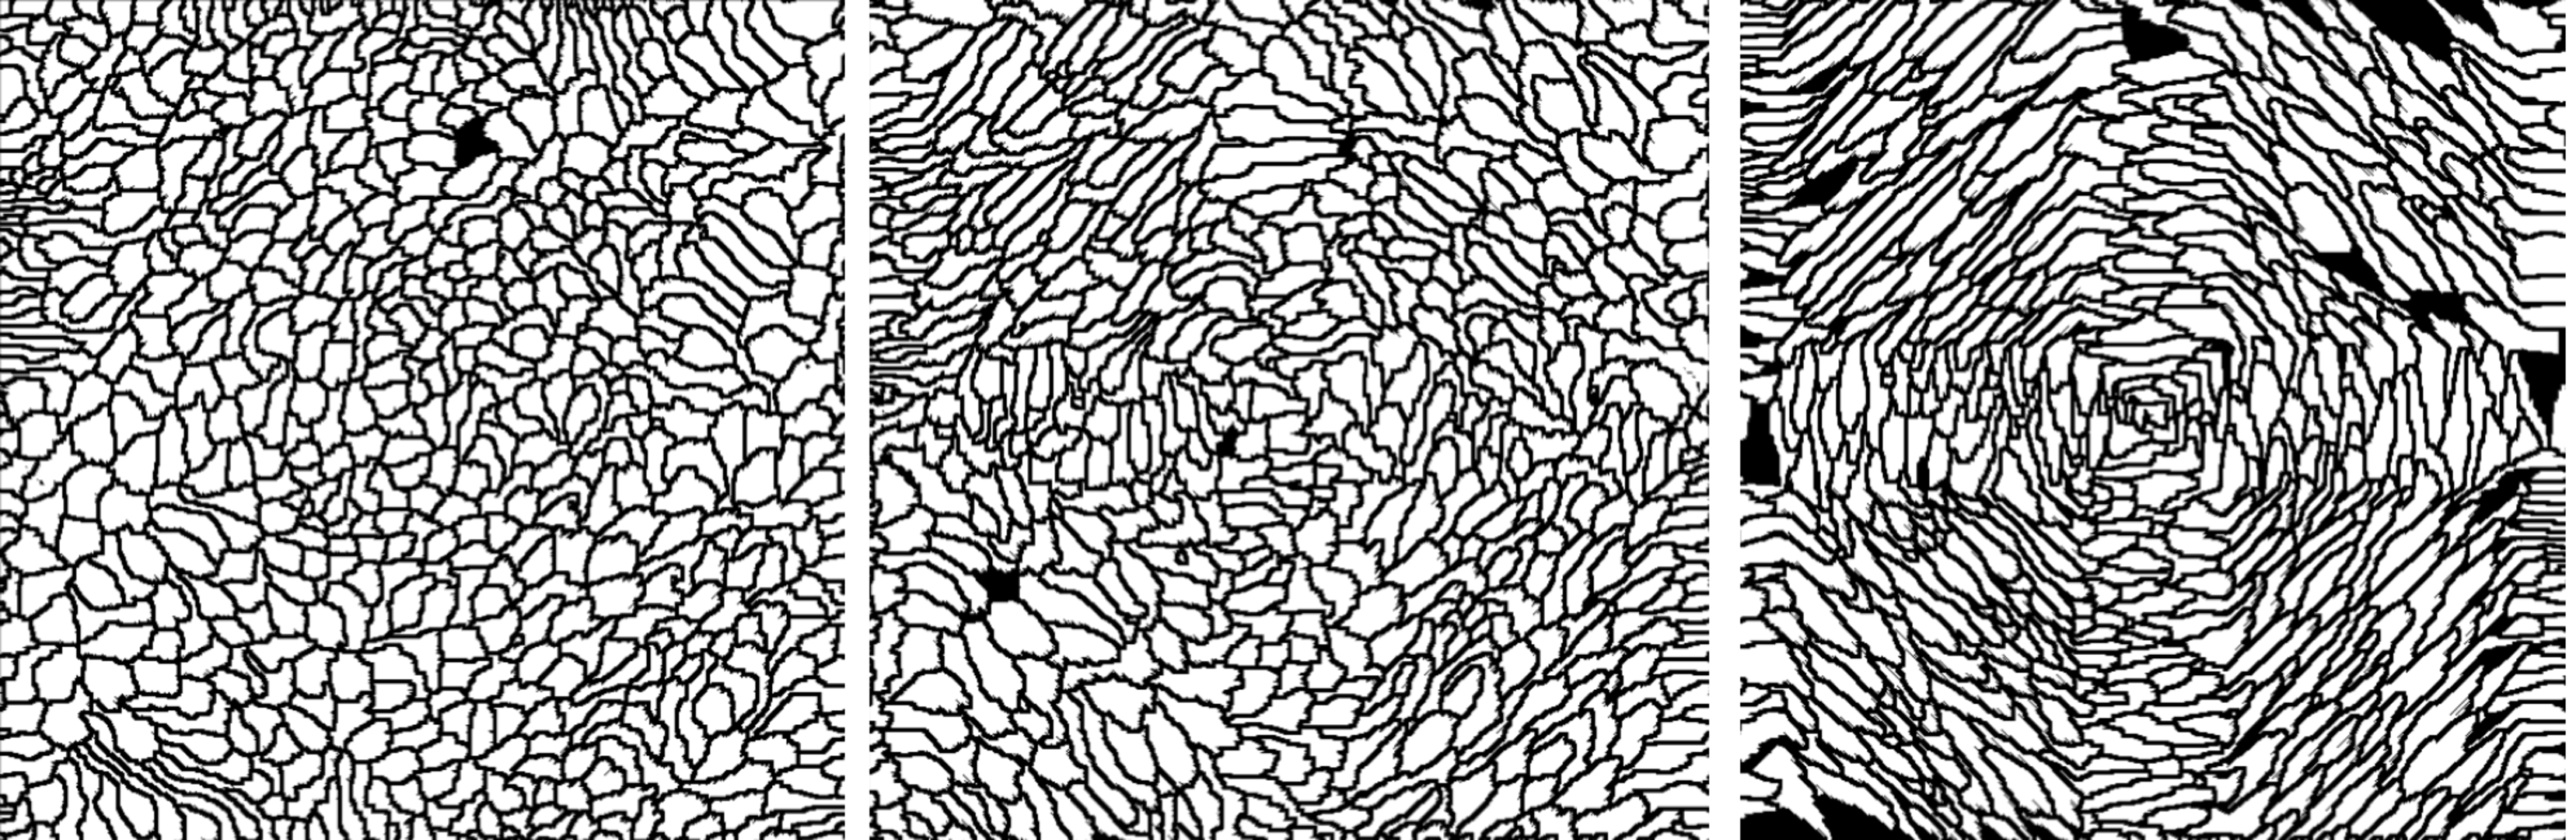
\includegraphics[width=12cm]{../figures/Fig3}
\end{frame}

\begin{frame}{Condiciones de contorno}
Geometrías tridimensionales \textbf{arbitrarias}.

\begin{itemize}
\item Se elige un eje Cartesiano ($x$, $y$ o $z$) y se computan cortes bidimensionales sobre ese eje.
\item Para cada corte se establecen condiciones de contorno, a través de un campo vectorial discreto que ``sigue'' al contorno
\end{itemize}

\textbf{Ortogonal al gradiente del corte}.

  \centerline{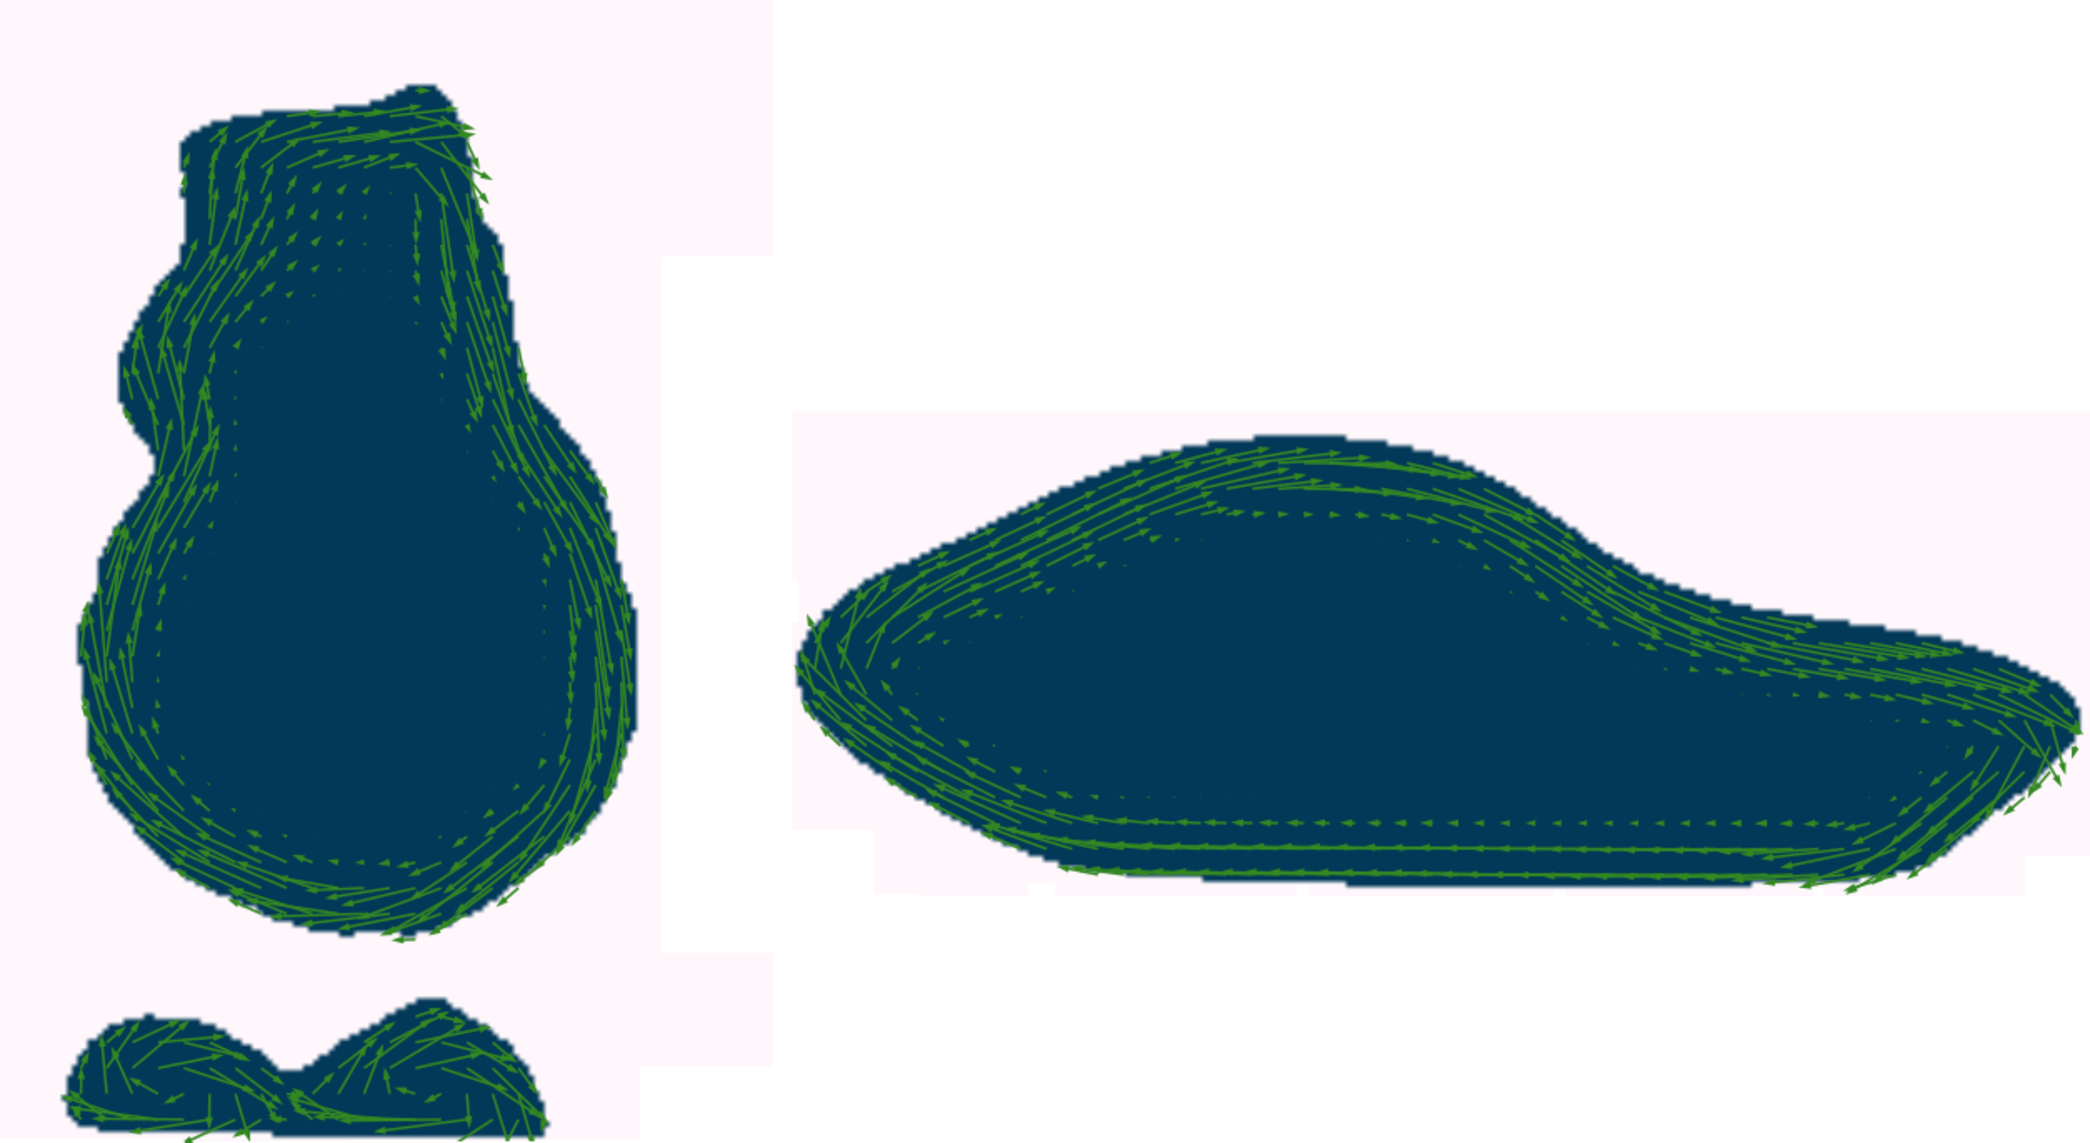
\includegraphics[width=7cm]{../figures/Fig4}}
\end{frame}

\subsection{Resultados}

\begin{frame}{Resultados}
Centrado del SD en el {\em centro de masa} de cada corte

Parametrización bidimensional (más intuitiva).

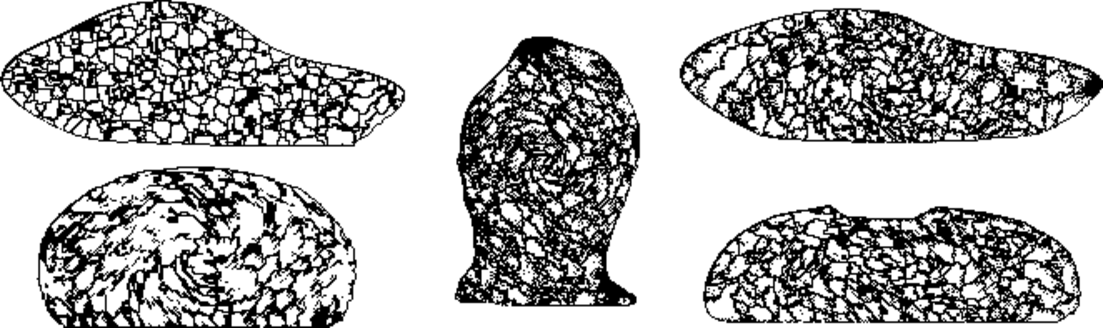
\includegraphics[width=12cm]{../figures/Fig5}
\end{frame}


\begin{frame}{Resultados}
Parámetro {\em separación} = 2 entre partículas

\centerline{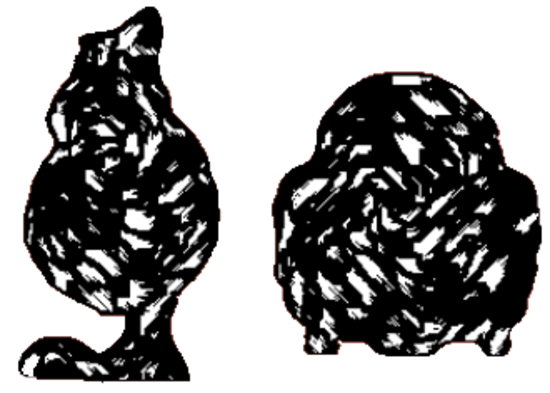
\includegraphics[width=8cm]{../figures/Fig7}}
\end{frame}

\begin{frame}{Resultados}
\centerline{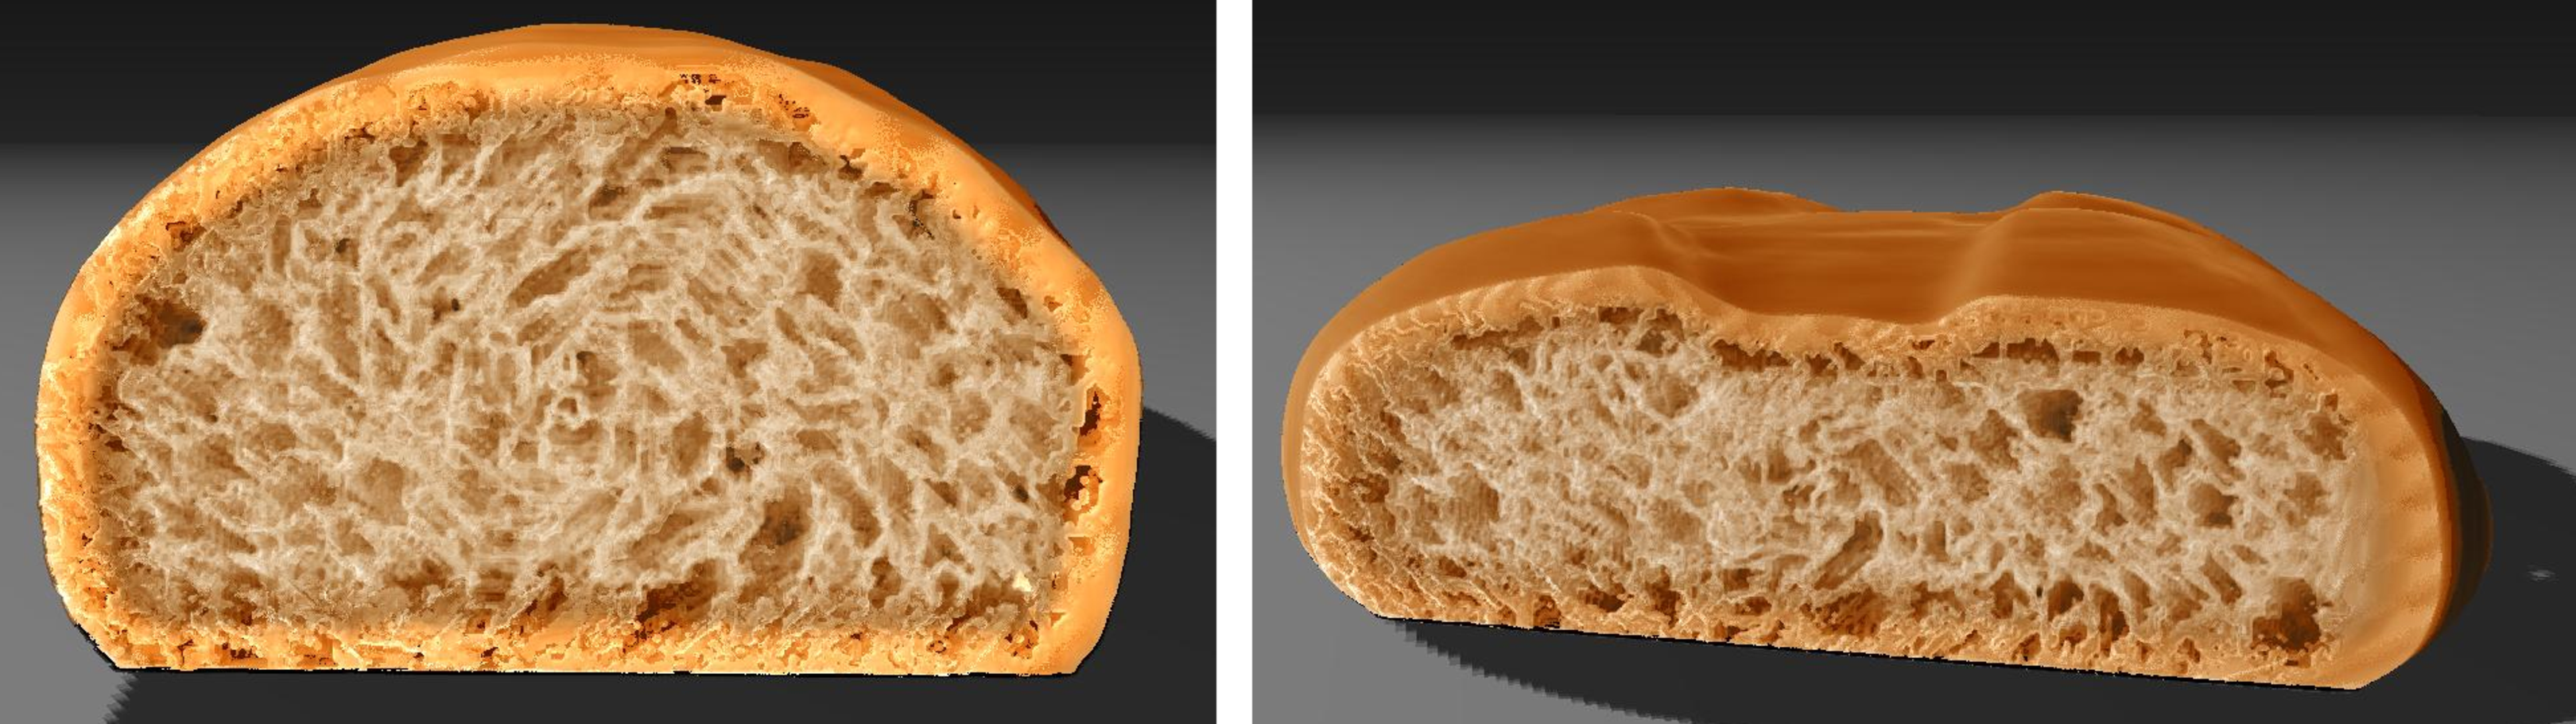
\includegraphics[width=10cm]{../figures/Fig11CAVW}}


Sistemas dinámicos adaptativos (dependiendo del ancho y alto del corte).

\centerline{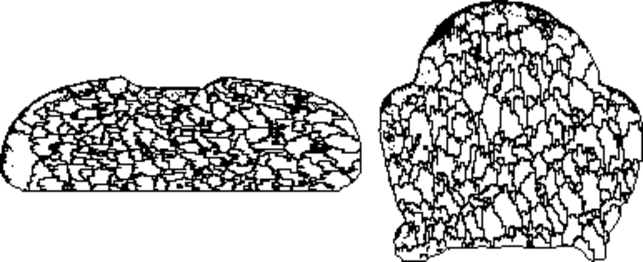
\includegraphics[width=7cm]{../figures/Fig6}}

\end{frame}


\begin{frame}{Renderizados}

\centerline{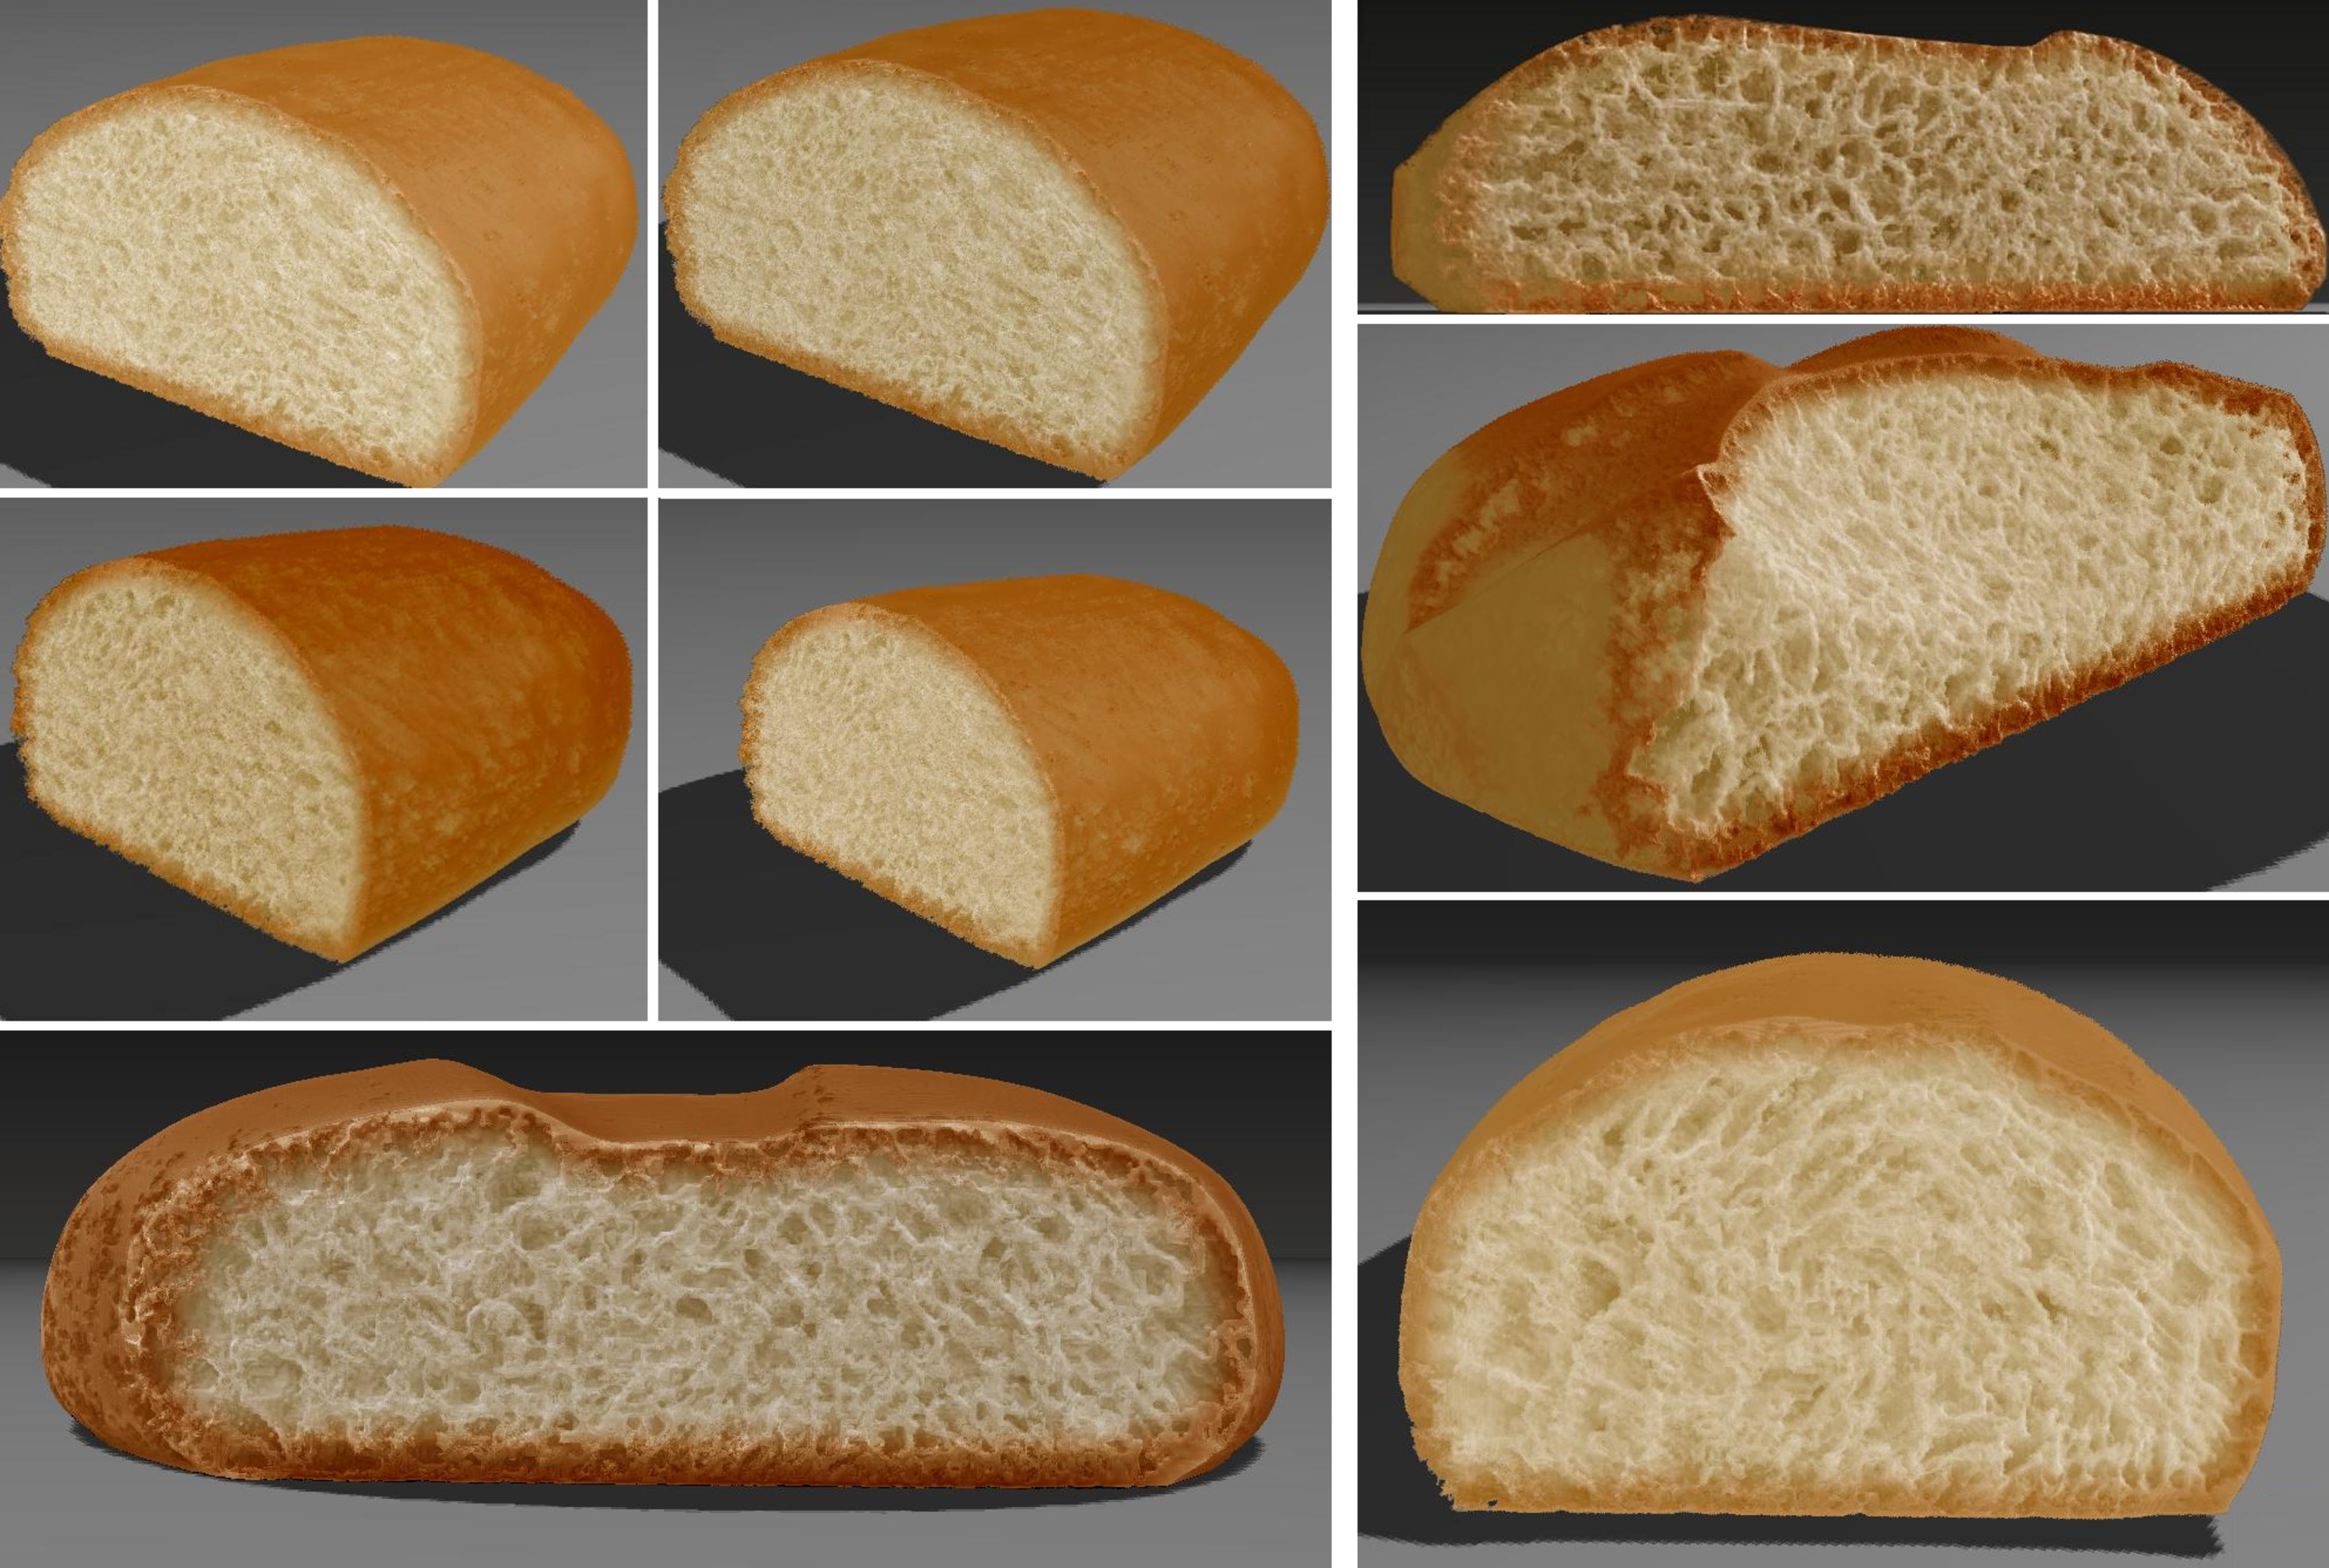
\includegraphics[width=10cm]{../figures/Fig12CAVW}}
\end{frame}

\begin{frame}{}

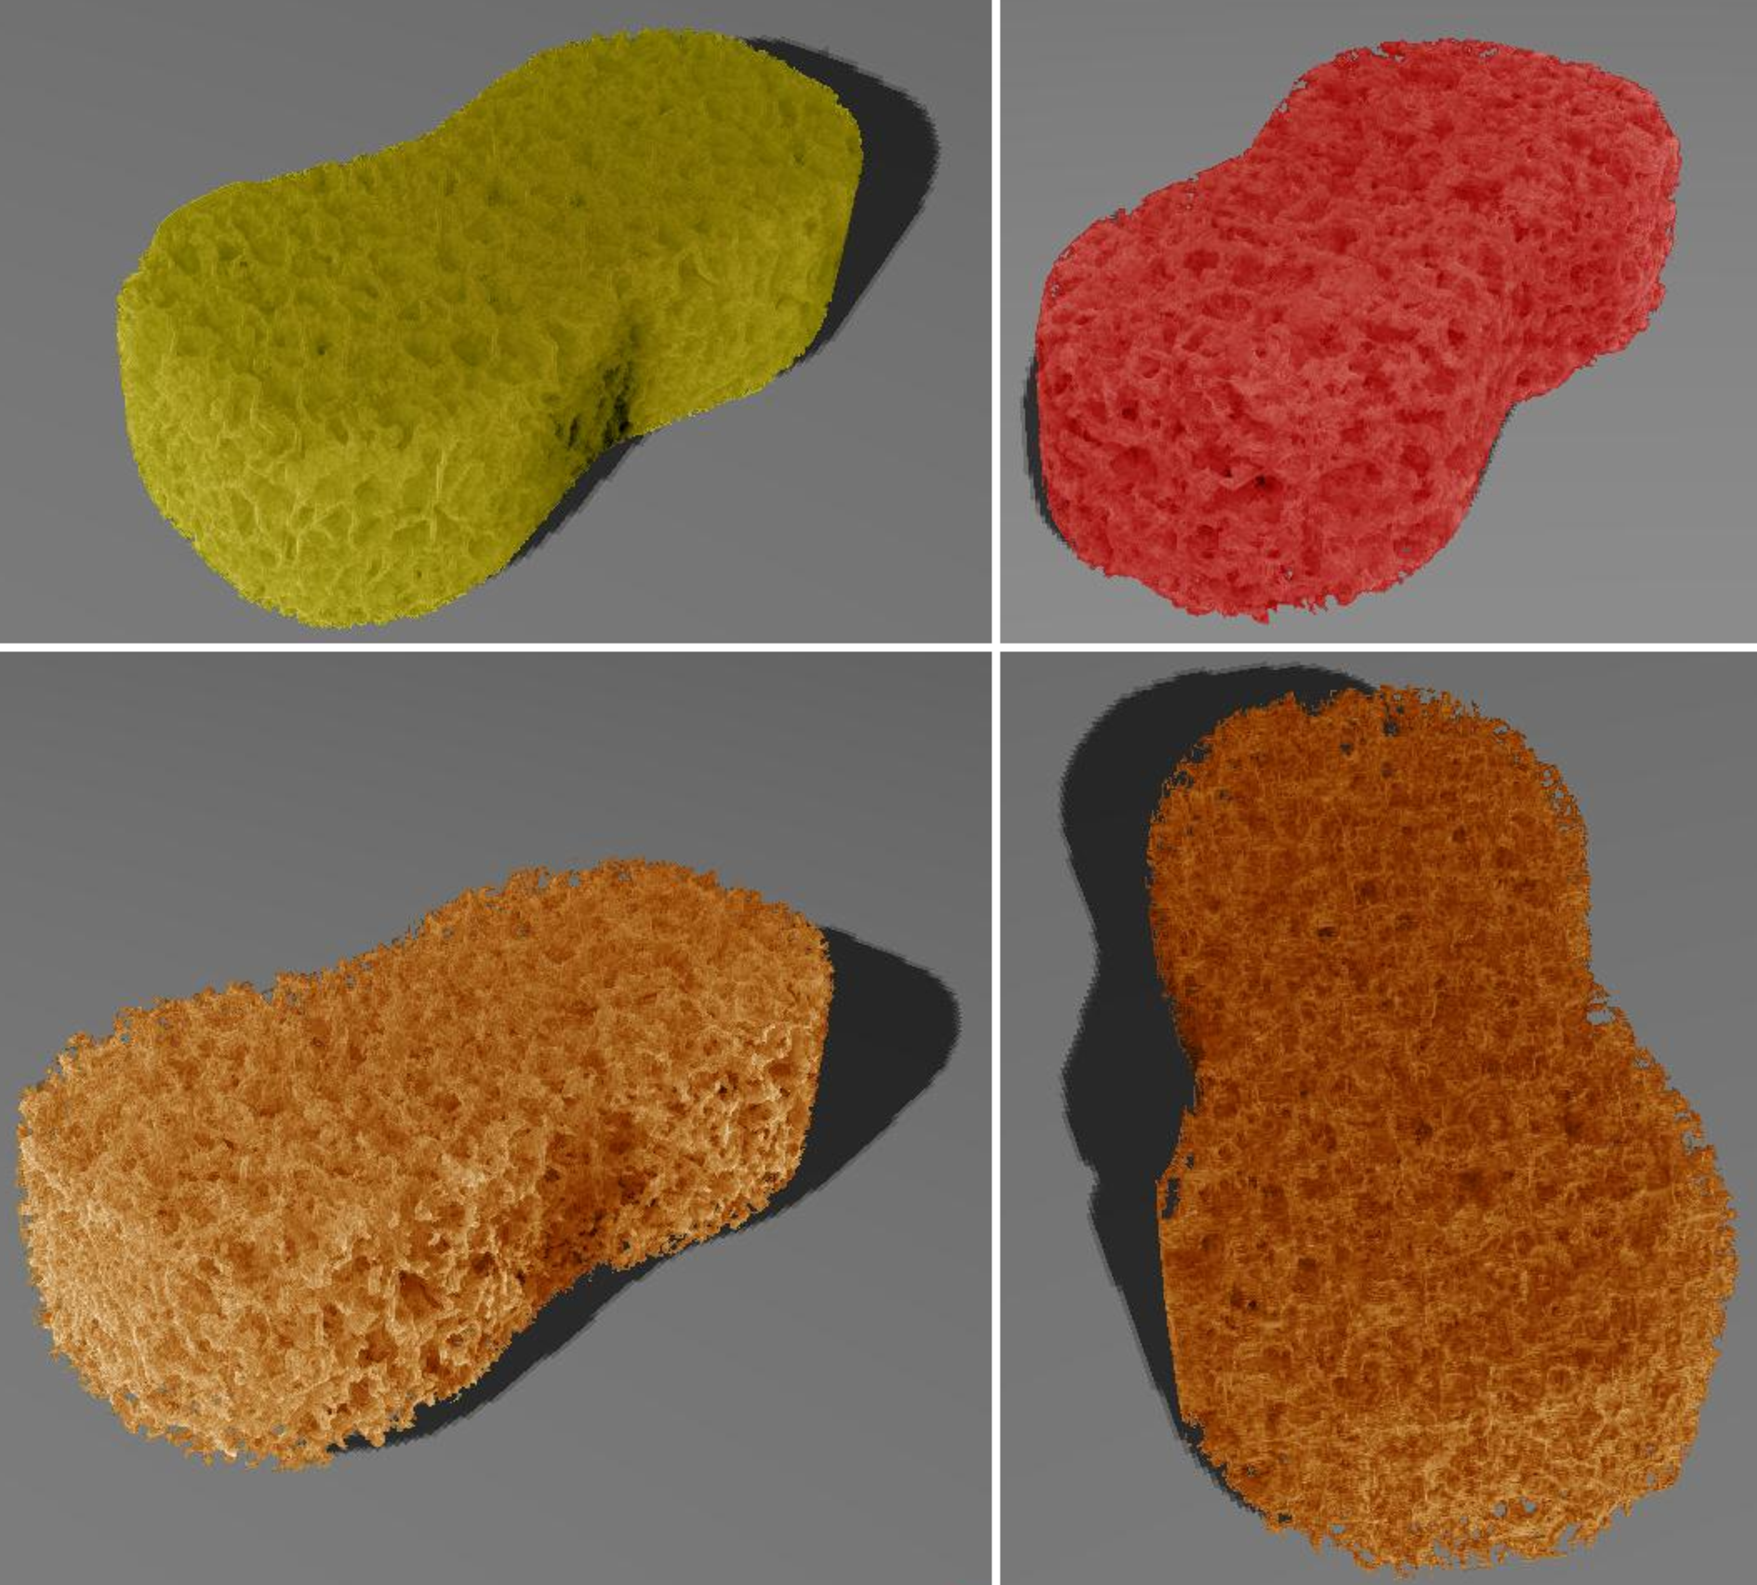
\includegraphics[width=6cm, height=7cm]{../figures/Fig13CAVW}
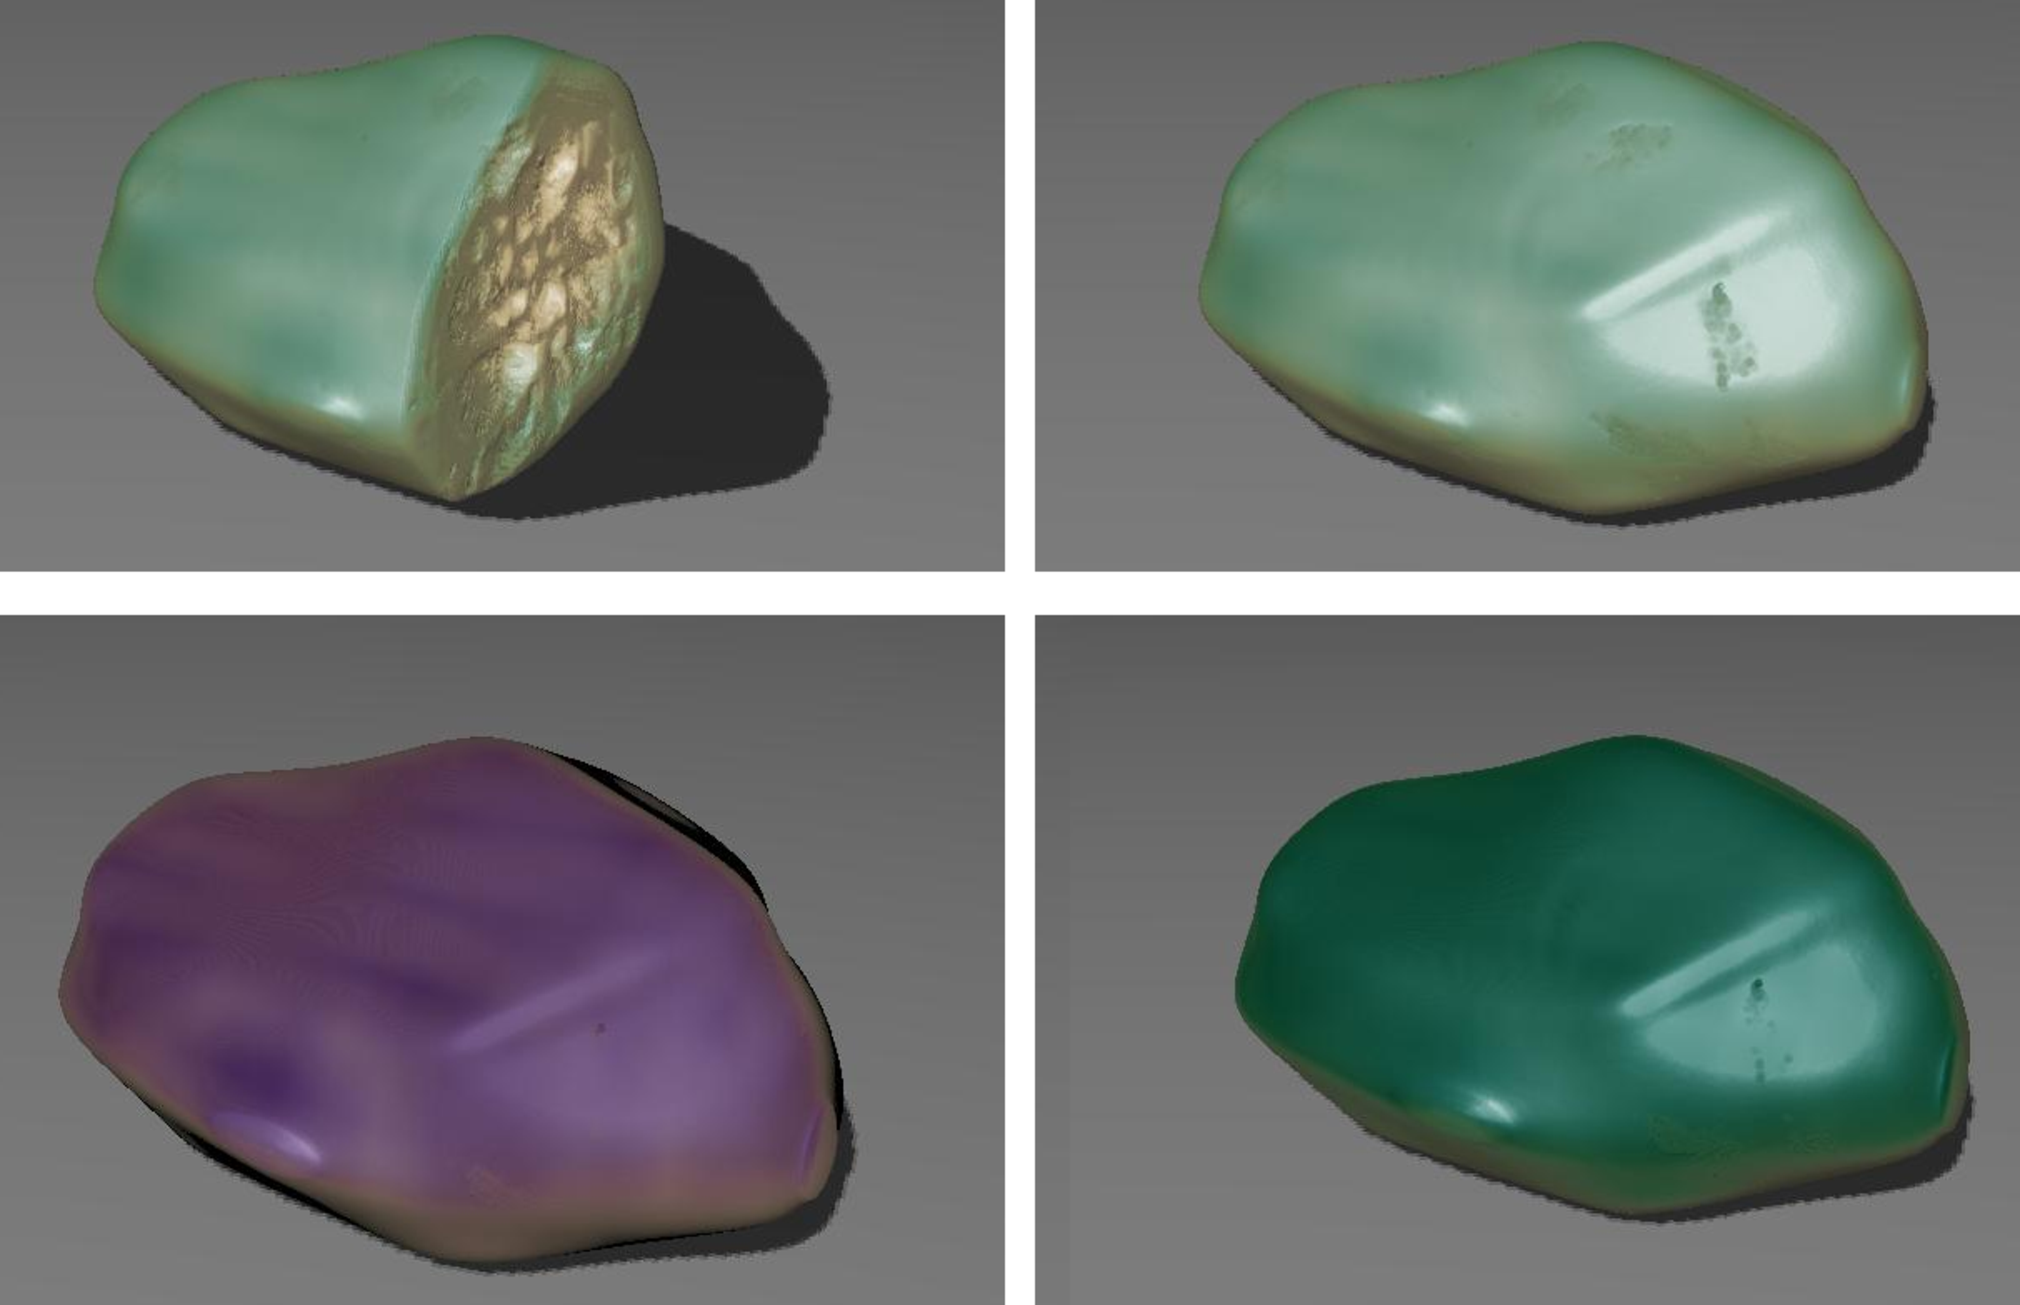
\includegraphics[width=6cm, height=6cm]{../figures/Fig14CAVW}

\end{frame}

\begin{frame}{Conclusiones}
\begin{block}{}
\begin{itemize}
\item Algoritmo procedimental fenomenológico
\item Resultados adecuados para computación gráfica
\item Permite representar diversos materiales porosos
\item No requiere esfuerzo por parte del usuario

\item Dificultad al controlar los sistemas dinámicos
\end{itemize}
\end{block}
\end{frame}


\section[Modelado de Pan]{Modelado procedimental de pan inspirado en su proceso de formación}


\begin{frame}
\begin{block}{}
\begin{center}
\vspace{1cm}
\huge{Modelado procedimental de pan inspirado en su proceso de formación}
\vspace{1cm}
\end{center}
\end{block}
\end{frame}

\subsection{Modelado procedimental de pan inspirado en su proceso de formación}
\begin{frame}{Modelado procedimental de pan inspirado en su proceso de formación}
\begin{block}{}
\begin{itemize}
\item Debido a la complejidad del proceso, el mismo ha sido ignorado en gran medida en la literatura de computación gráfica.

\item Sin embargo, ha sido ampliamente estudiado en ingeniería de los alimentos.

\item No existe aún un modelo unificado (cocción, leudado, formación de la corteza, etc.).

\item Subproceso $\rightarrow$ algoritmo procedimental.
\end{itemize}
\end{block}
\end{frame}

\begin{frame}{Propuesta}
\centerline{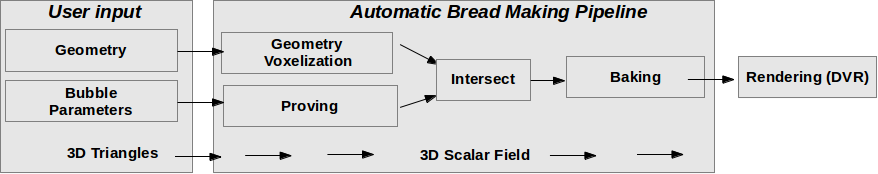
\includegraphics[width=12cm]{../figures/pipeline}}
\end{frame}

\begin{frame}{Leudado}
Simulación por \textbf{extracción de esferas} de un cubo

$N(r)$: cantidad de esferas extraídas (inversamente proporcional al radio $r$ de la esfera). Ley fractal:

\begin{equation*}
N(r) = \frac{k}{r^{d}}
\end{equation*}

\vspace{0.3cm}
\centering
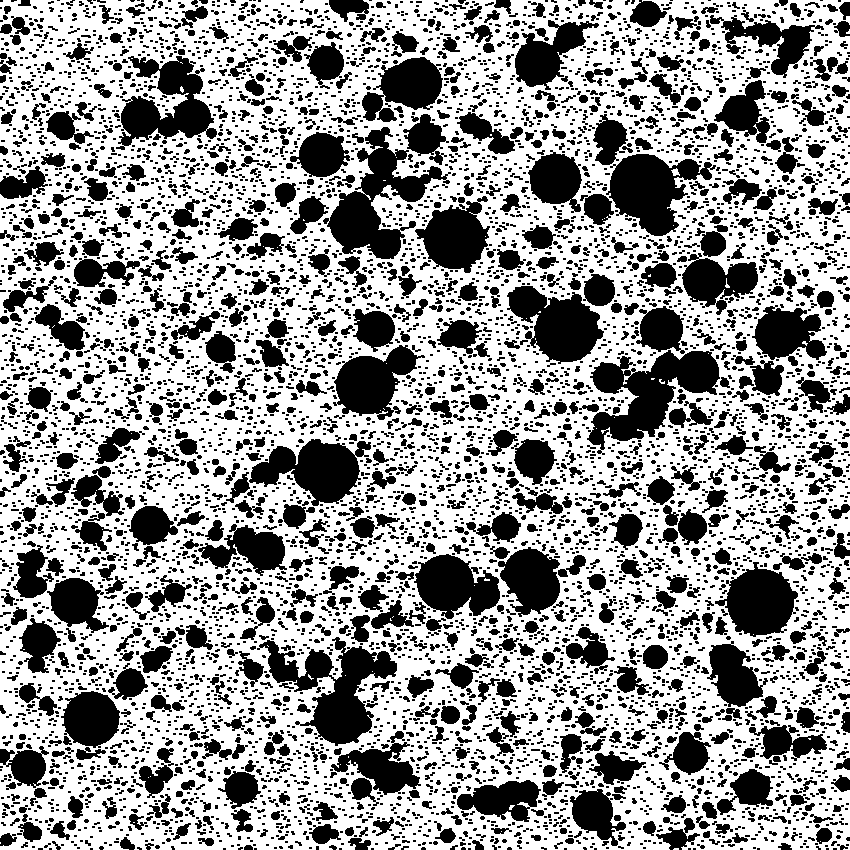
\includegraphics[height=3.5cm]{../figures/bubbles}
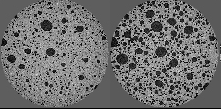
\includegraphics[height=3.5cm]{../figures/proving}
\end{frame}

\begin{frame}
Intersección de burbujas $\rightarrow$ estructura no necesariamente fractal

%\vspace{1cm}

\centering
Burbujas $\cap$ Geometría

Enmascarado directo (multiplicación)

\centerline{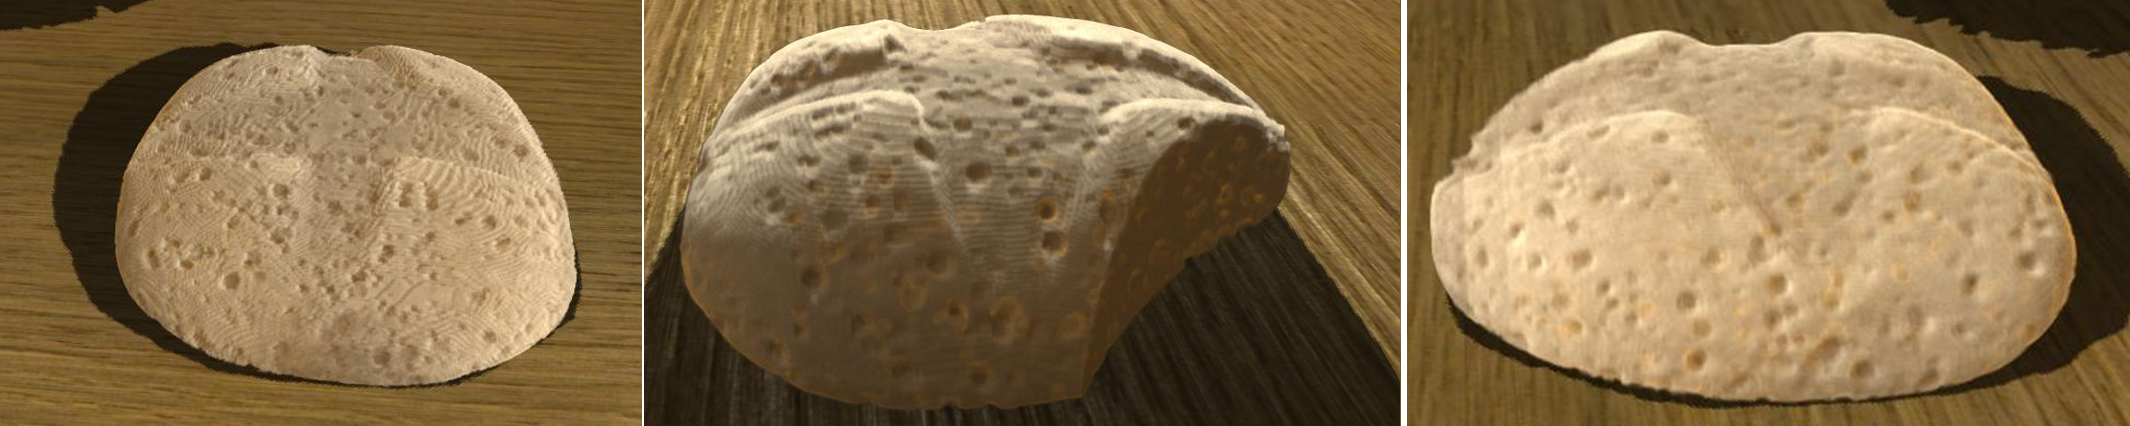
\includegraphics[width=8cm]{../figures/intersectProblem}}
%\end{frame}

%\begin{frame}{Mapa de Distancias}

%Textura volumétrica a valores reales $DF_{M}$ con las mismas dimensiones que la entrada $M$,


%$$DF_{M}[i,j,k] = \min \bigg\{ \delta([i,j,k],[i',j',k']): M[i',j',k'] = 0 \bigg\},$$


%\begin{itemize}
%\item $[i,j,k]$ y $[i',j',k']$ son celdas en las respectivas texturas (posiciones espaciales $(i,j,k)$ y $(i',j',k')$)
%\item $\delta$ es la función que computa la distancia entre dos celdas (distancia de Manhattan, Euclidiana).
%\end{itemize}

%\end{frame}

%\begin{frame}{Solución: \textbf{Mapa de Distancias}}
Solución: \textbf{Mapa de Distancias}
\centerline{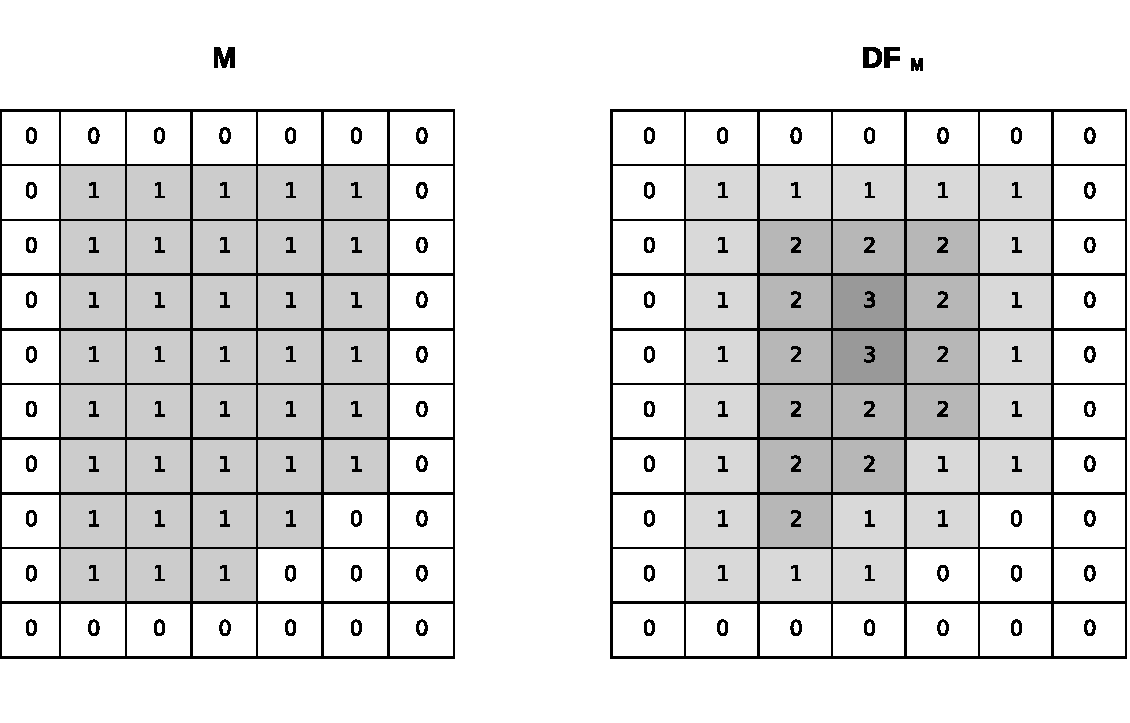
\includegraphics[width=7cm]{../figures/DistanceTransform}}

\end{frame}

\begin{frame}
\textbf{Umbral} DF $\rightarrow$ corteza de ancho \textbf{parametrizable}.

\vspace{0.3cm}

\centerline{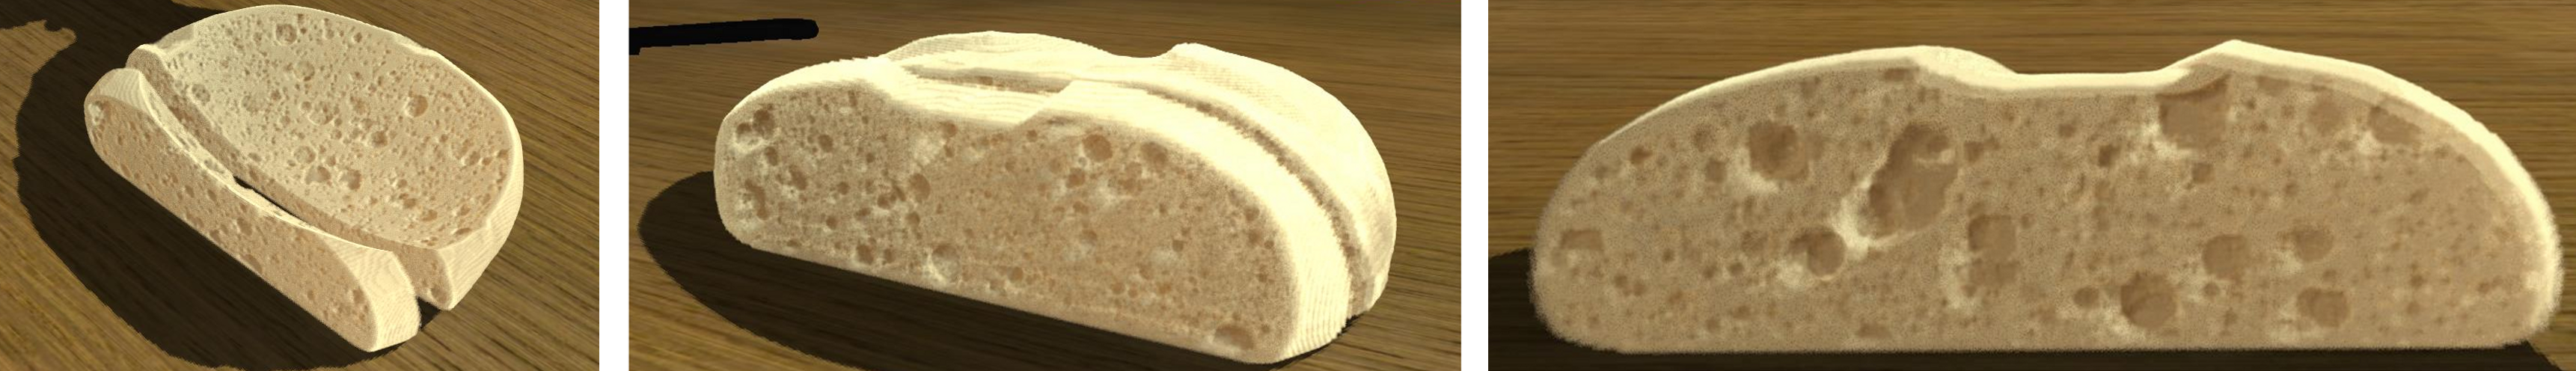
\includegraphics[width=10cm]{../figures/prebakebread}}

\centerline{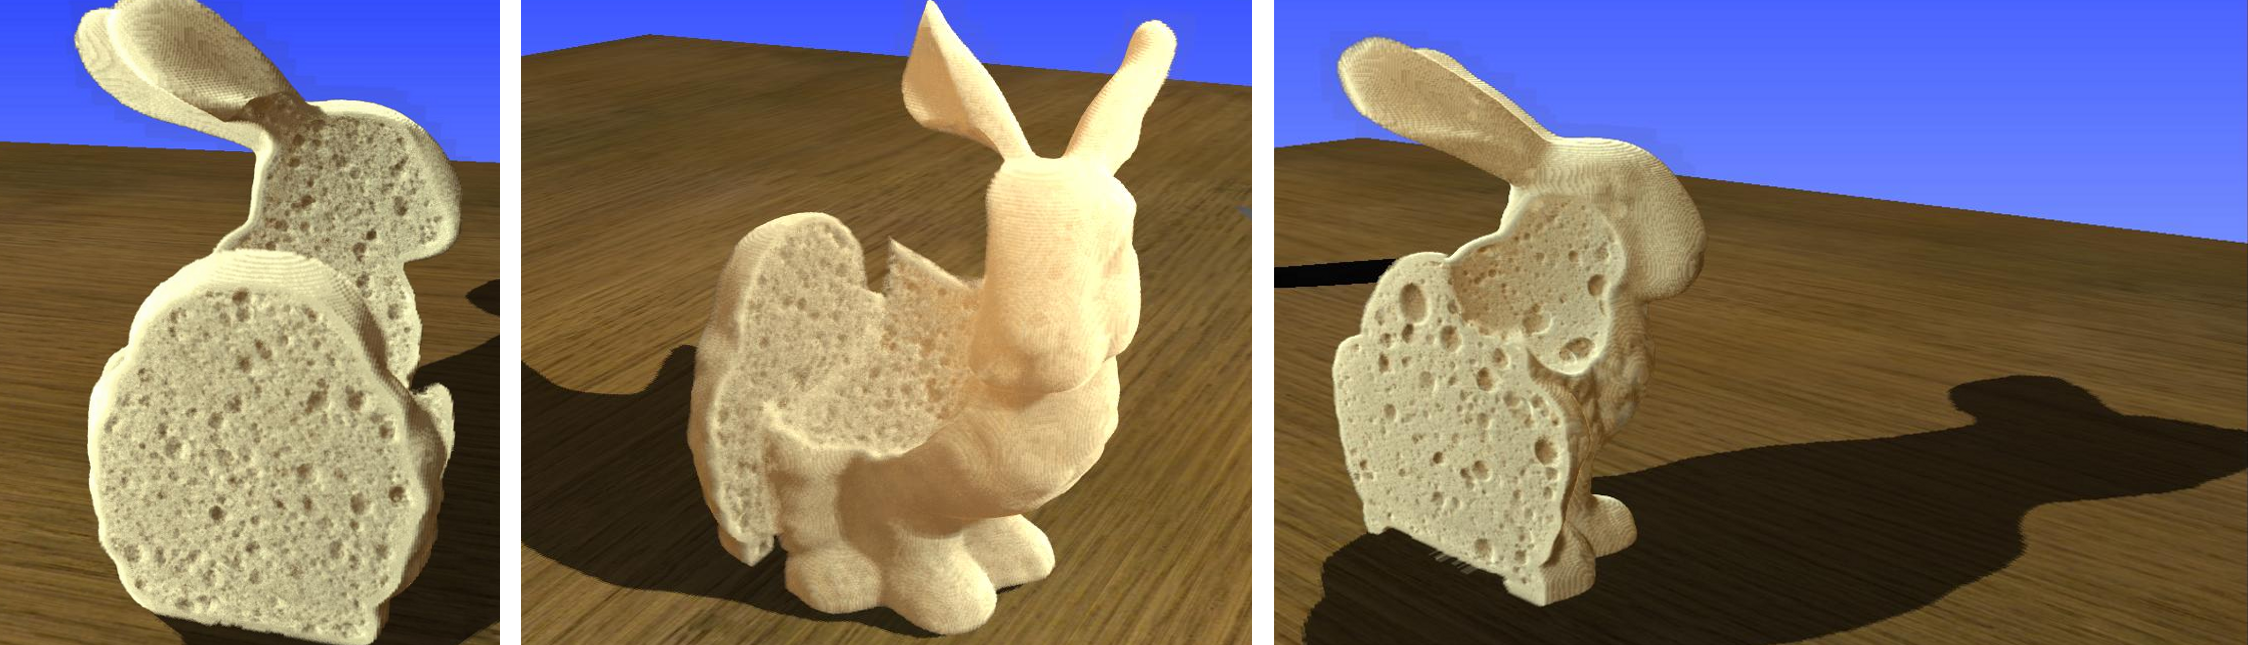
\includegraphics[width=10cm]{../figures/prebakebunny}}
\end{frame}

\subsection{Cocción}

\begin{frame}{Cocción}
Procesos durante la cocción:

\begin{itemize}
\item Transferencia de calor y masa
\item Crecimiento de las burbujas
\item Deformación de la masa original
\item Formación de la corteza
%\item Reacciones químicas
\end{itemize}

En nuestro caso, debe atenderse especialmente al efecto de dichos procesos sobre la \textbf{apariencia}.

%\end{frame}

%\begin{frame}{Cocción}

Cocción $3D$:

\begin{itemize}
\item Costoso
\item Complejo
\end{itemize}


Modelo $1D$:

\begin{itemize}
\item Se obtienen soluciones similares para nuestros propósitos.
\end{itemize}


%\begin{equation}
%\label{Eq:heat}
%\frac{\partial T}{\partial t} = \frac{1}{\rho C_{p}} \frac{\partial}{\partial x} \left ( k \frac{\partial T}{\partial x} \right ) + \frac{\lambda}{C_{p}} \frac{\partial W}{\partial t}+\frac{\lambda W}{ \rho C_{p} }\frac{\partial \rho}{\partial t},
%\end{equation}
%
%\noindent donde

%$T$ temperatura, $x$ es la coordenada radial, $t$ tiempo, $C_{p}$ calor específico, $\rho$ densidad, $k$ conductividad térmica, $\lambda$ calor latente de la evaporación de agua, y $W(x,t)$ contenido de agua líquida.

%Condiciones iniciales:
%\begin{align*}
%T(x,0) &= T_{0}(x), 0\le x \le L/2,
%\end{align*}

\end{frame}

%\begin{frame}{Cocción}
%Condiciones de borde (continuidad y suavidad)
%\begin{align*}
%\left ( \frac{\partial T}{\partial x} \right )_{x=L/2} &= 0 , t > 0 \\
%-k \left ( \frac{\partial T}{\partial x} \right )_{x=0} &= h_{r}(T_{r}-T_{s}) + h_{c}(T_{air}-T_{s}) - \lambda \rho D_{w} \left (\frac{\partial W}{\partial x} \right )_{x=0}
%\end{align*}
%

%\end{frame}

\begin{frame}

$Temp$: Arreglo \textbf{unidimensional} de temperaturas.


Distribución 3D de la temperatura utilizando el DF:
\begin{equation*}
\displaystyle R_{vol}[x,y,z] = Temp[ round( DF_{M}[x,y,z] ) ], 
\end{equation*}

$DF_{M}[(x,y,z)] = 0 \rightarrow$ contorno, $Temp[0] \rightarrow R_{vol}[(x,y,z)]$.
$DF_{M}[(x,y,z)] > 0 \rightarrow$ interior, $<$ T  $\rightarrow R_{vol}[(x,y,z)]$.

\centerline{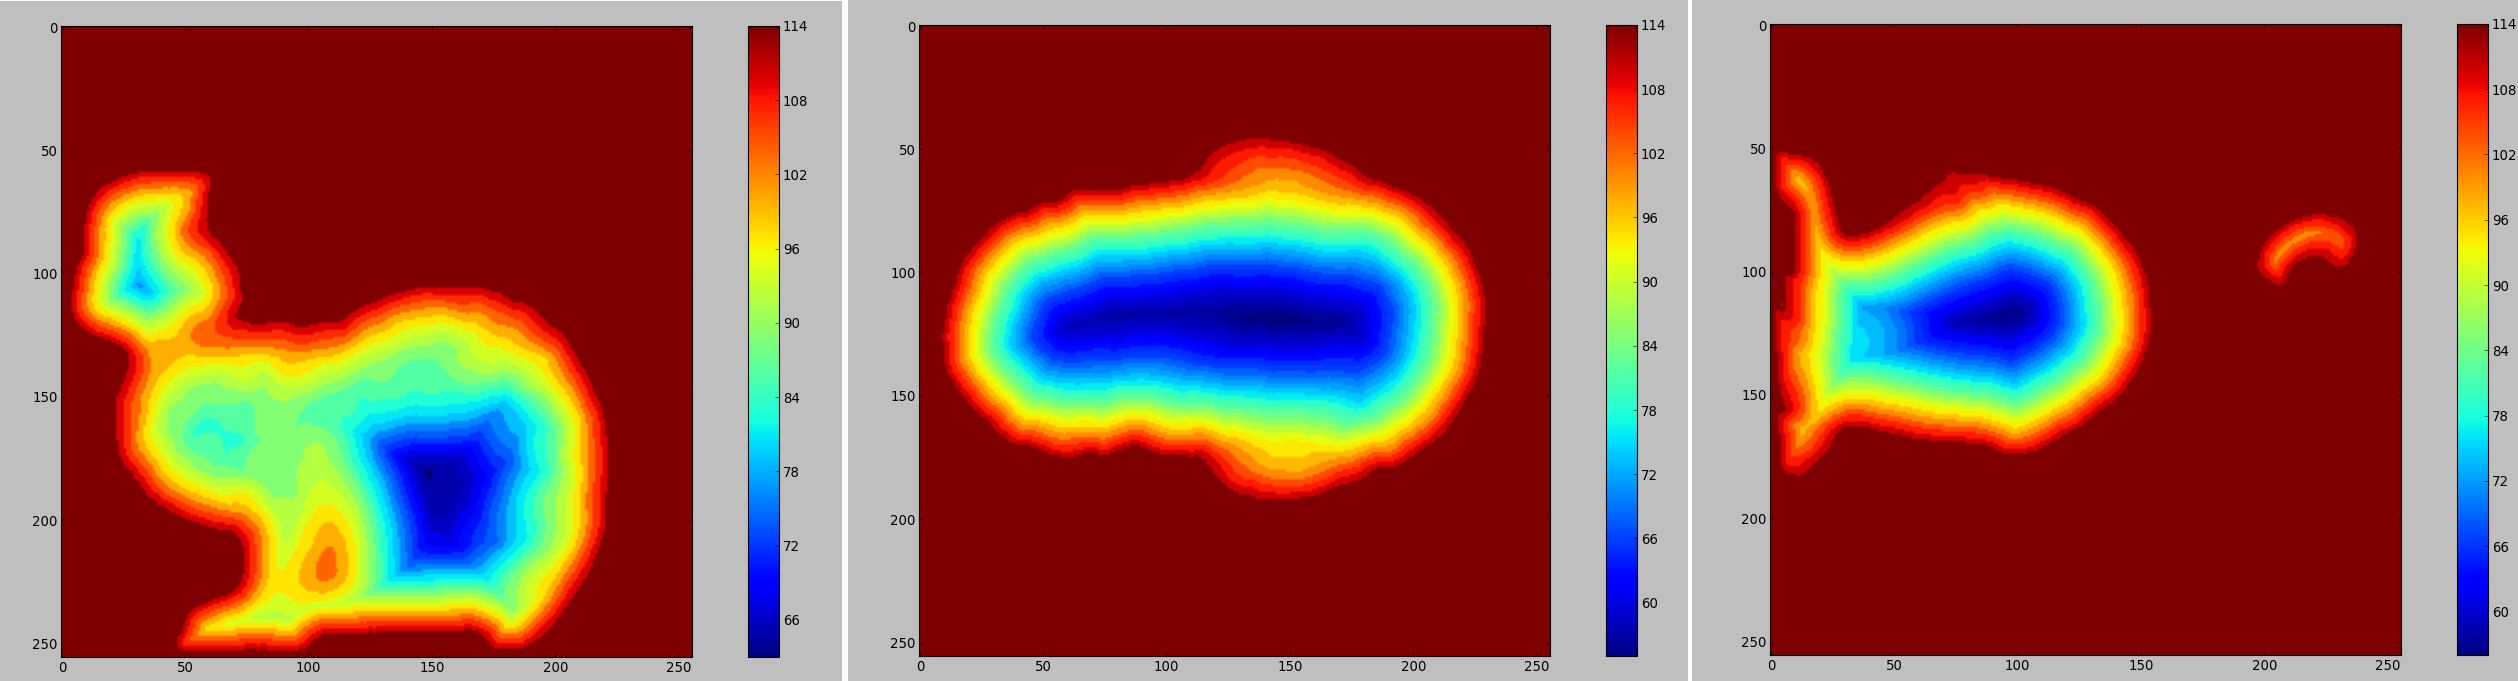
\includegraphics[width=8cm]{../figures/tempsbunny}}
\end{frame}

\begin{frame}{Deformación por Temperatura}

Operación de \textbf{warping}: deforma burbujas de acuerdo a la temperatura (3D, dirección de crecimiento, SD).

\begin{align*}
\displaystyle
[x,y,z] = [u,v,w] + p\, g'[u,v,w],
\end{align*}

$g' = gauss(\nabla R_{vol})$

$p = 5,10,15$:
\centerline{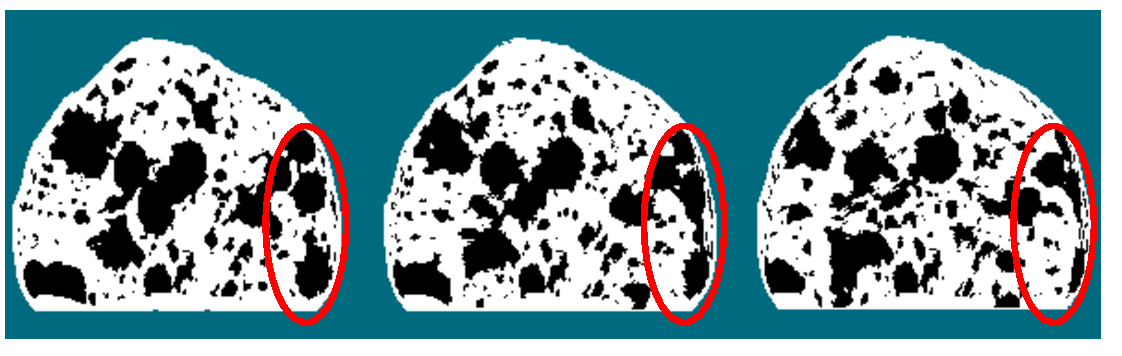
\includegraphics[width=11cm]{../figures/parameterp}}

\end{frame}

\begin{frame}{Levantamiento de la masa}

\textbf{Distribución} de burbujas durante el leudado

\begin{equation*}
P[x,y,z] = max \bigg\{r\bigg\}
\end{equation*}

(mayor burbuja en $[x,y,z]$)

\vspace{0.2cm}

Deformación \textbf{local}: $p = P[u,v,w],$

\begin{equation*}
[r,s,t] = [u,v,w] + P[u,v,w] \, g'[u,v,w],
\end{equation*}

%\noindent donde $[u,v,w]$ es la entrada original, y $[r,s,t]$ es la coordenada deformada.


Escalado de la textura (de acuerdo a la distribución de burbujas)


\begin{equation*}
[x,y,z] = [r,s,t]\, S \, P[r,s,t],
\end{equation*}

\end{frame}

\begin{frame}{Resultados}

\centerline{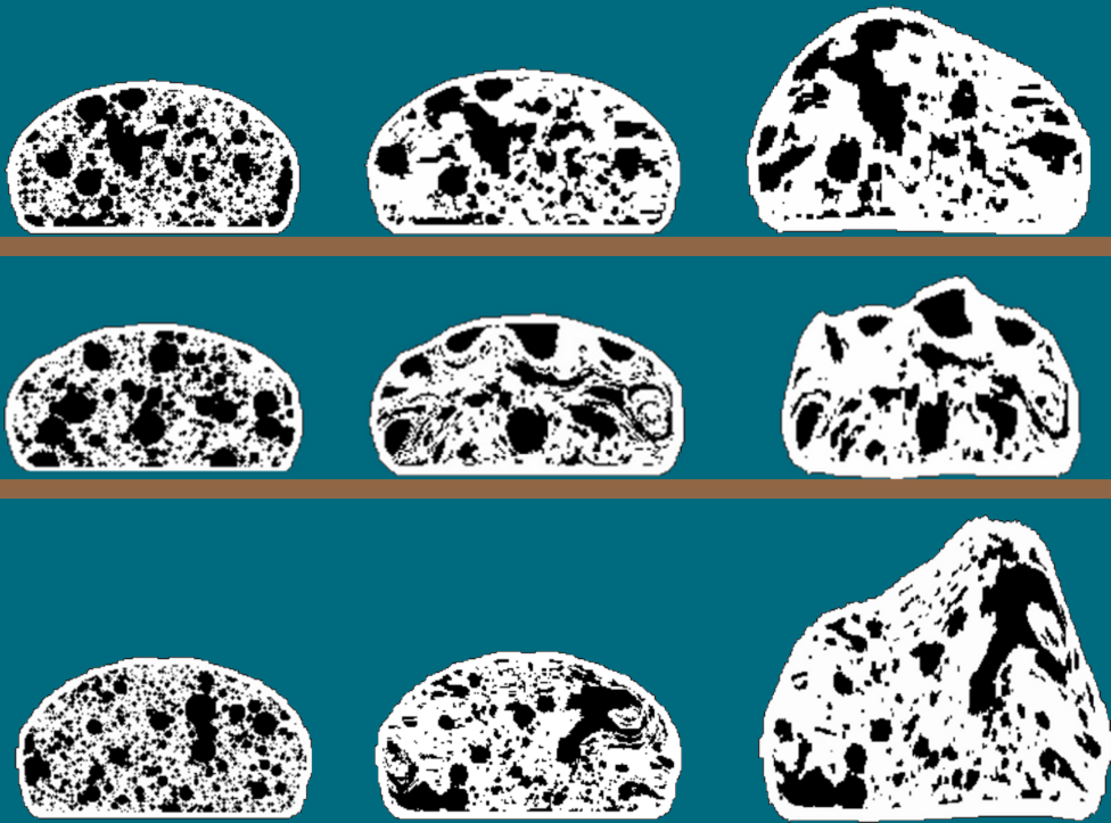
\includegraphics[width=9cm]{../figures/Fig9}}

\end{frame}

\begin{frame}{Corteza}
Colores CIELab de muestras reales, reportadas por Purlis et. al. (2009).

\begin{align*}
L &= 40 \rightarrow \text{máxima cocción}\\
L &= 90 \rightarrow \text{sin cocción}
\end{align*}

\centerline{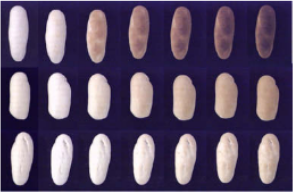
\includegraphics[width=4cm]{../figures/browning}}

%\end{frame}

%\begin{frame}

%Los valores de los canales $a$ y $b$ no están reportados. A partir de fotografías se observa que varian suavemente al cambiar $L$.

%\vspace{0.2cm}

{\em \textbf{Densidad} de la corteza}: $N_{v} / W_{size} \rightarrow L$

\begin{itemize}
\item $N_{v}$ número de voxels $= 1$ en una ventana en el entorno de la posición,
\item $W_{size}$ número de voxels en esa ventana.
\end{itemize}

\vspace{0.2cm}
Los colores se distribuyen de acuerdo al valor de $L$. $<$ masa $\Rightarrow < L$.

\end{frame}


\subsection{Resultados}

\begin{frame}{Resultados}

\centerline{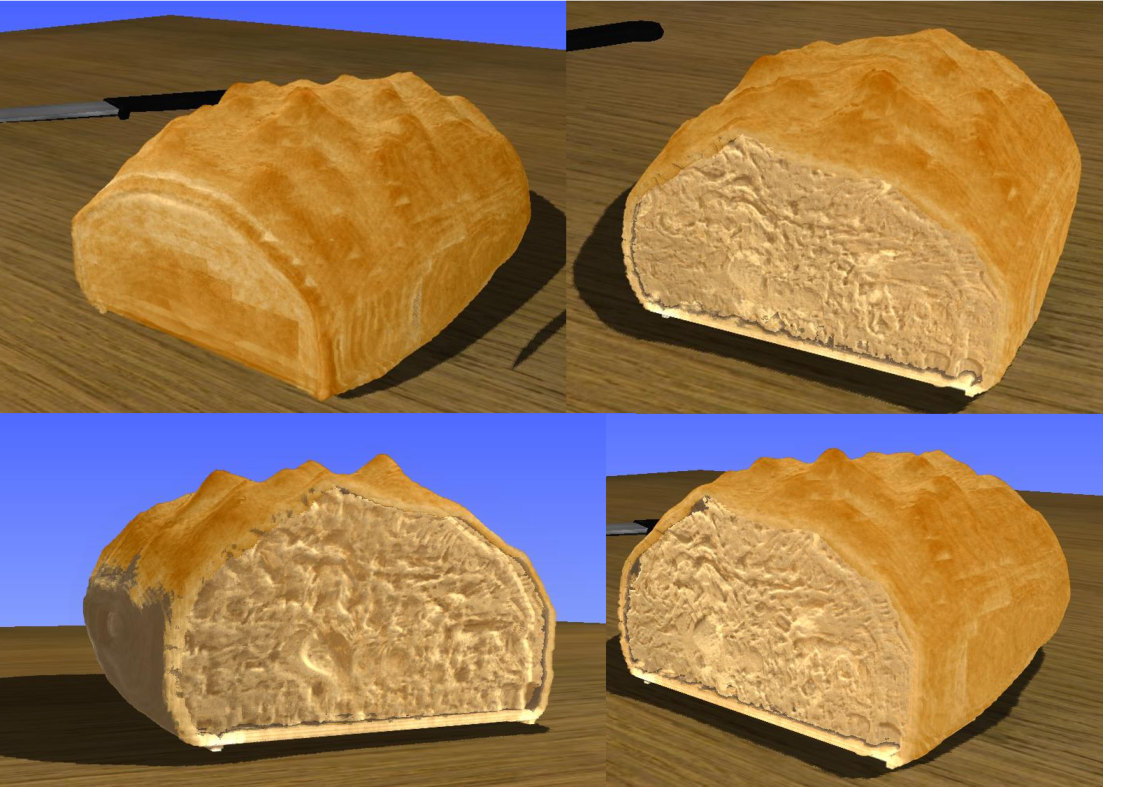
\includegraphics[width=9cm]{../figures/Fig11}}

$S$ con valores aleatorios en cada punto, picos visibles en la corteza.

\end{frame}

\begin{frame}{Resultados}

\centerline{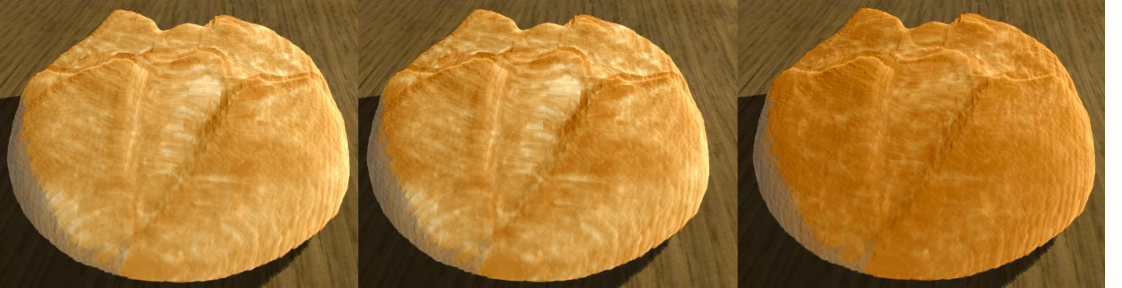
\includegraphics[width=12cm]{../figures/Fig13}}
Cortezas con diferentes historias de cocción. De izquierda a derecha, se decrementa el valor máximo admitido para el canal $L$.

\end{frame}

\begin{frame}{Resultados}
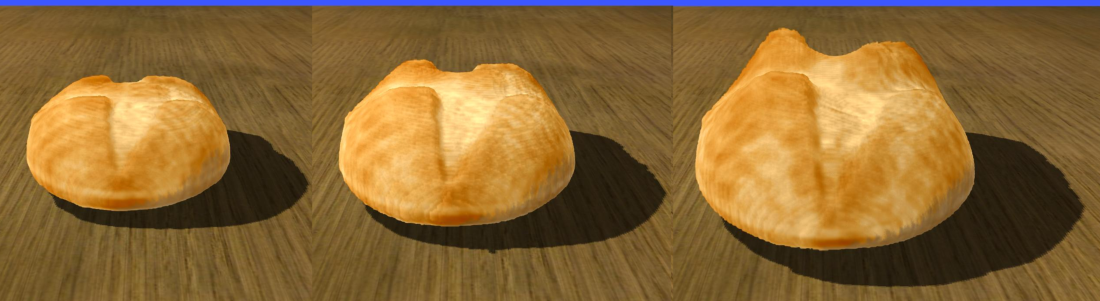
\includegraphics[width=11cm]{../figures/Fig14}

Panes luego de la cocción mostrando diferentes crecimientos. De izquierda a derecha se incrementa el parámetro $S$.

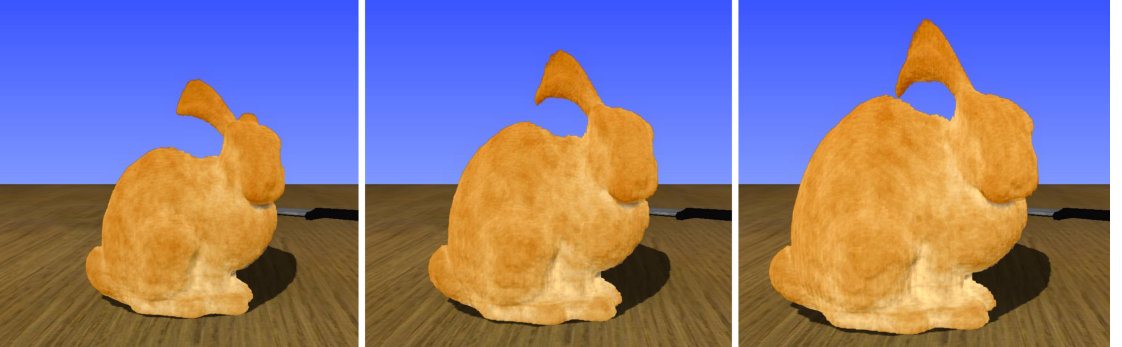
\includegraphics[width=9cm]{../figures/Fig15}


\end{frame}

%\begin{frame}{Tiempos de Cómputo}

%\begin{table}[h!]
%\begin{tabular}{lllll}
%\hline\noalign{\smallskip}
%Resolución de la Textura Volumétrica & $256^{3}$ & $384^{3}$  & $512^{3}$ \\
%\noalign{\smallskip}\hline\noalign{\smallskip}
%Leudado & 3.62 & 12.07 & 31.29 \\
%Intersección & 8 & 10.27 & 14.97 \\
%Transformación de Distancia & 7 & 23.73 & 56 \\
%Cocción  & 49.81 & 144.69 & 313.7 \\
%\hline\noalign{\smallskip}
%Total & 68.43 & 190.76 & 415.96 \\
%Rendering & 1s & 4s & 0\% \\
%\noalign{\smallskip}\hline
%\end{tabular}
%\caption{Tiempos de cómputo típicos de las distintas etapas de la fabricación sintética de pan, expresados en segundos.}
%\label{tab:computingtimes}
%\end{table}
%\end{frame}

\begin{frame}{Conclusiones}
\begin{block}{}
\begin{itemize}
\item Modelo \textbf{inspirado} físicamente
%\item Elimina decisiones ad-hoc
\item Se simula cocción, levantamiento de la masa, etc.
\item Permite obtener imágenes en sucesivas etapas del proceso de formación
\end{itemize}
\end{block}
\end{frame}

\section{Renderización}


\begin{frame}
\begin{block}{}
\begin{center}
\vspace{1cm}
\huge{Renderización}
\vspace{1cm}
\end{center}
\end{block}
\end{frame}


\subsection{Renderización}

\begin{frame}{Renderización}

Muchas técnicas de renderizado utilizan \textbf{mallas} para computar los resultados (vértices, y conexiones entre ellos)

\ \\

En nuestro caso, se propone

\textbf{textura volumétrica} $\rightarrow$ \textbf{Renderizado Directo de Volúmenes}

\begin{itemize}
\item Evita construcción de una malla.
\item Permite \textbf{cortes arbitrarios} del material (trivialmente).
\end{itemize}

\end{frame}

\begin{frame}{DVR}
DVR aproxima la Ecuación del Transporte Radiativo (RTE).

Se computa un \textbf{rayo} para cada pixel, desde la pantalla al objeto.

\textbf{Cambio de radiancia} del rayo a lo largo del medio.


\centerline{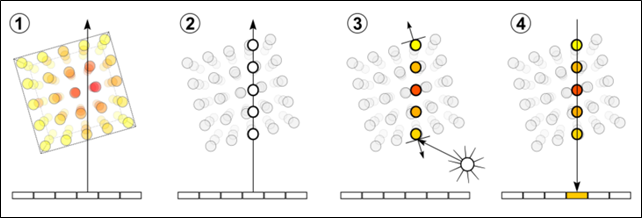
\includegraphics[width=9cm]{../figures/dvr}}

Para obtener resultados en tiempo real, tomamos una versión simplificada de la RTE, teniendo en cuenta solamente la \textbf{transmitancia}.
\end{frame}

%\begin{frame}{Renderización}



%\textbf{Transmitancia}: es la cantidad de luz que \texttt{atraviesa} un segmento del volumen:

%\begin{equation*}
%  T(p_i,p_j) = e^{-\tau_{(p_i, p_j)}}.
%\end{equation*}

%donde el \textbf{coeficiente de absorción} $ = \int_{p_i}^{p_j} k_a(t) \, dt$  $ = \tau_{(p_i, p_j)}$.



%\centerline{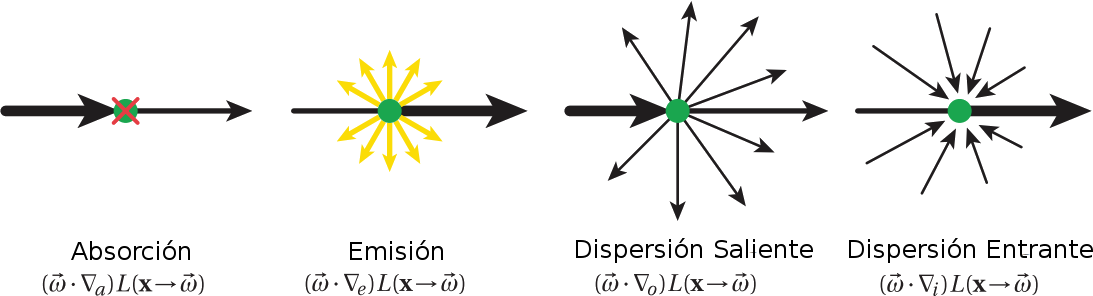
\includegraphics[scale = 0.25]{../figures/fenomenosrte}}


%\end{frame}

%\begin{frame}
%RTE sólo teniendo en cuenta transmitancia:

%\begin{equation*}
%  L(p_n) = L_b \ e^{-\tau(p_0, p_n)} + \int_{p_0}^{p_n} \rho \ e^{-\tau(t,p_n)} \, dt.
%\end{equation*}

%(Transmitancia de fondo $+$ Transmitancia del medio)

%La implementación reemplazará la integral por una suma,

%\begin{equation*}
%  L(p_n) = L_b \ e^{-\tau(p_0, p_n)} + \sum_{p_0}^{p_n} \rho \ e^{-\tau(p_i,p_n)}.
%\end{equation*}


%\end{frame}


\begin{frame}{DVR en GPU}

\begin{itemize}
\item Computamos un \textbf{rayo principal} desde la cámara hacia el volumen
\item \textbf{Sombras}: cada paso del rayo origina un \textbf{rayo secundario}, computando la transmitancia desde la posición actual hacia la luz
\end{itemize}

\centerline{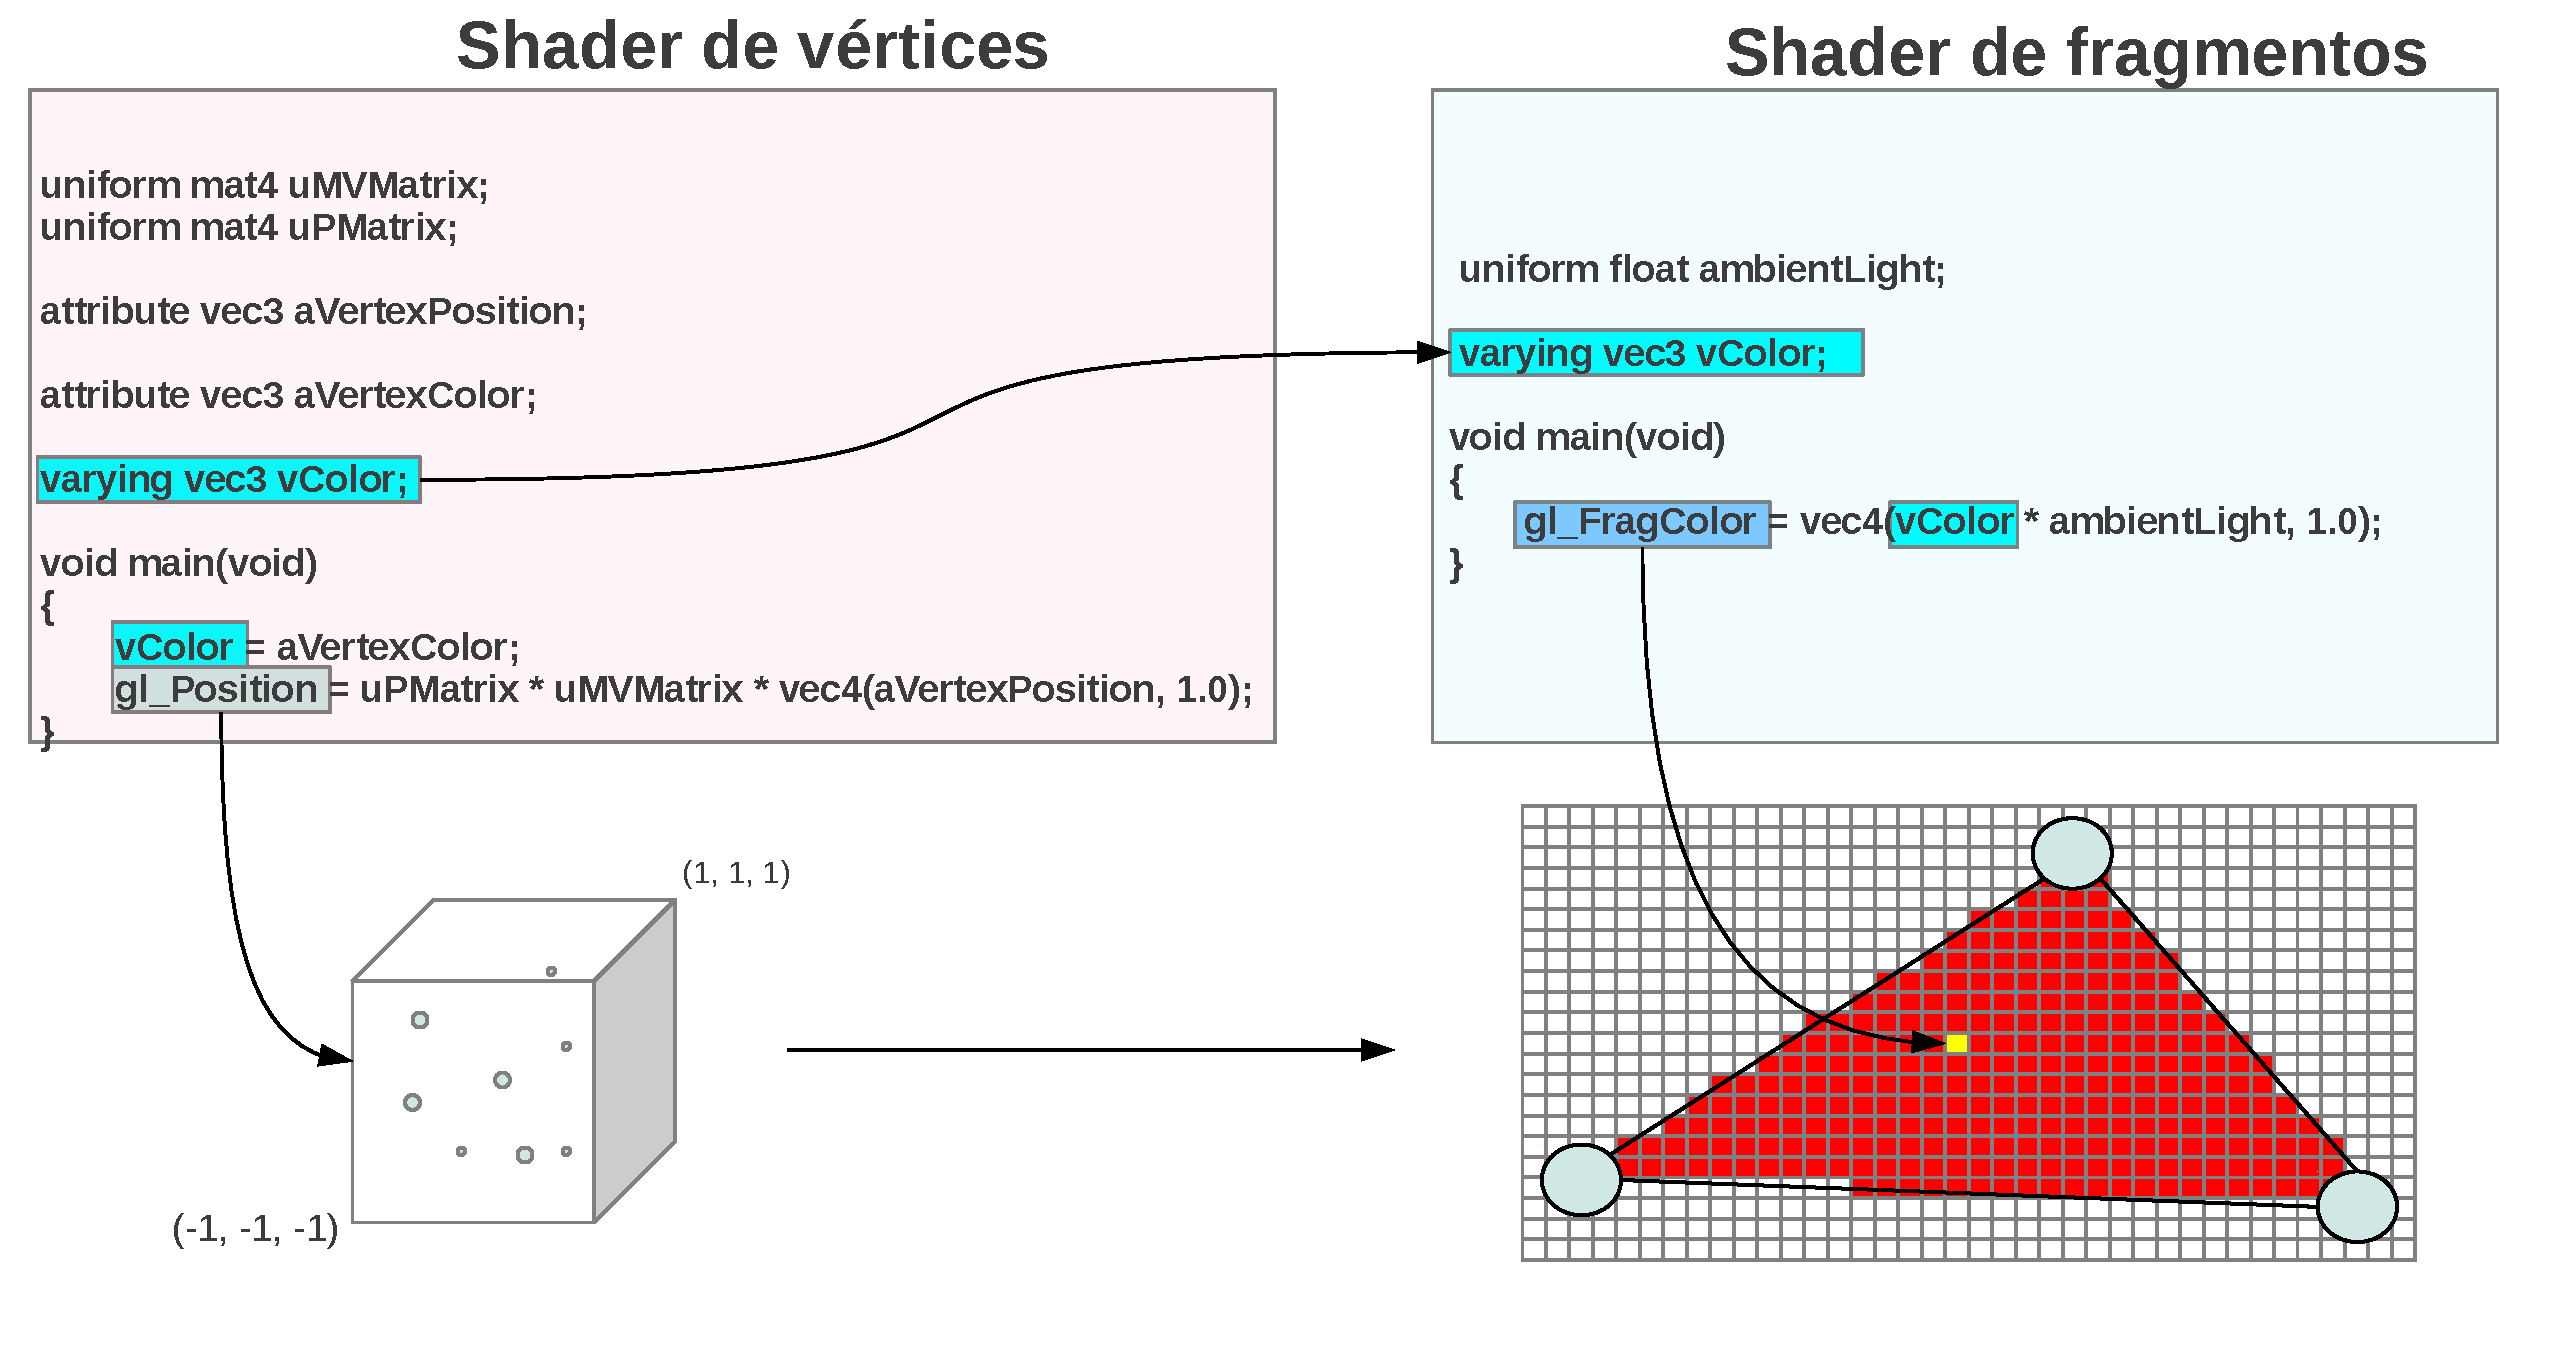
\includegraphics[width=4cm]{../figures/fragmentshader}}

\end{frame}

\begin{frame}
Implementación en GPU, (\textbf{fragment shader}, dentro del \textbf{pipeline gráfico}).

\centerline{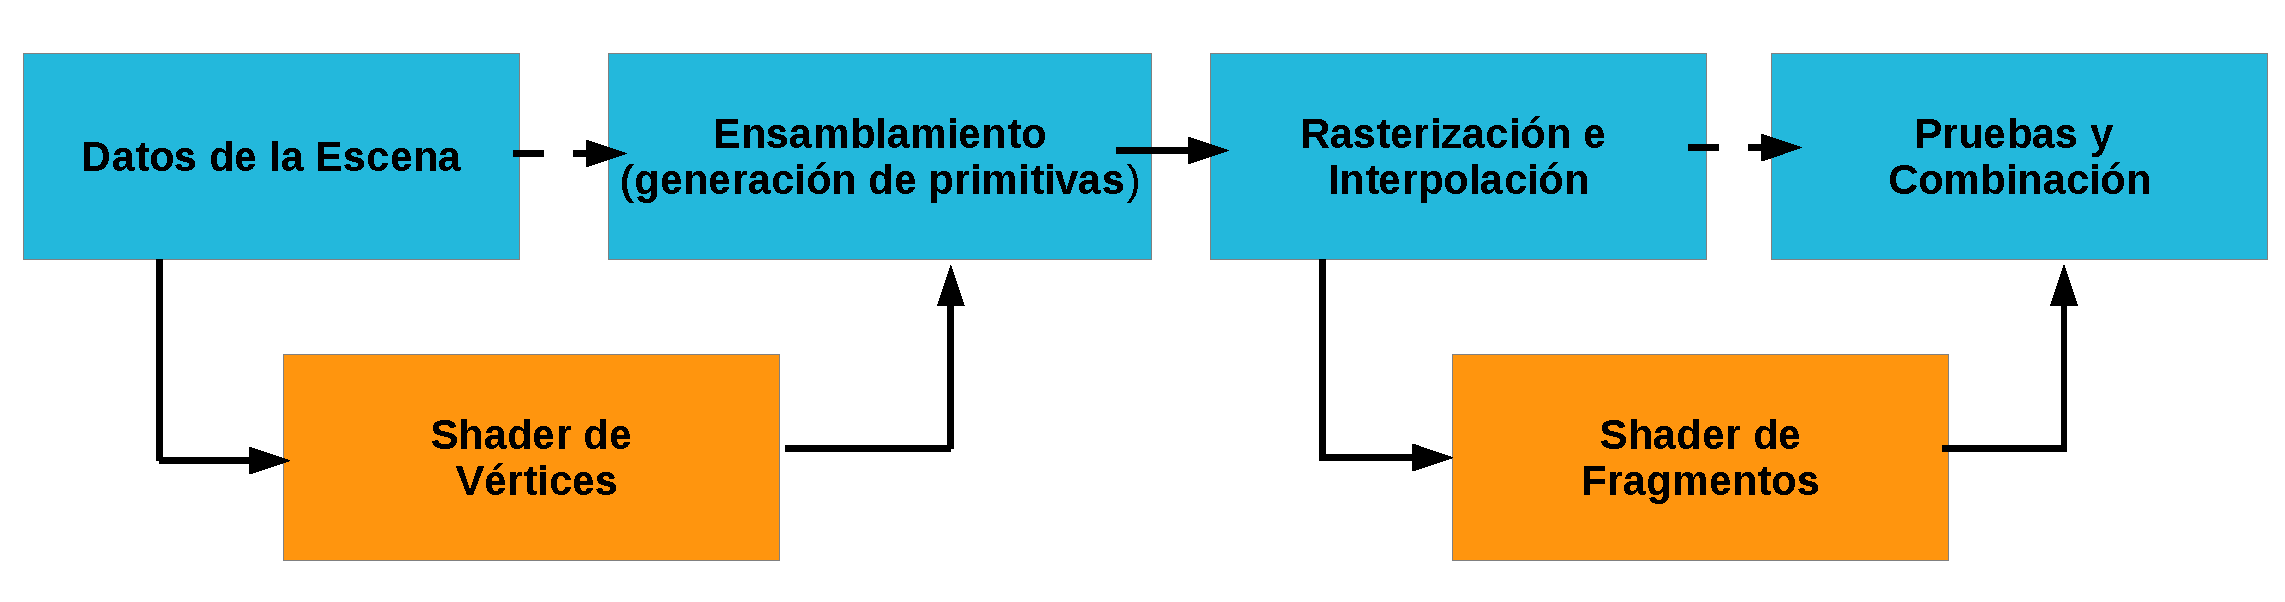
\includegraphics[width=13cm]{../figures/pipelinegrafico}}

\begin{table}[htb]
\centering
%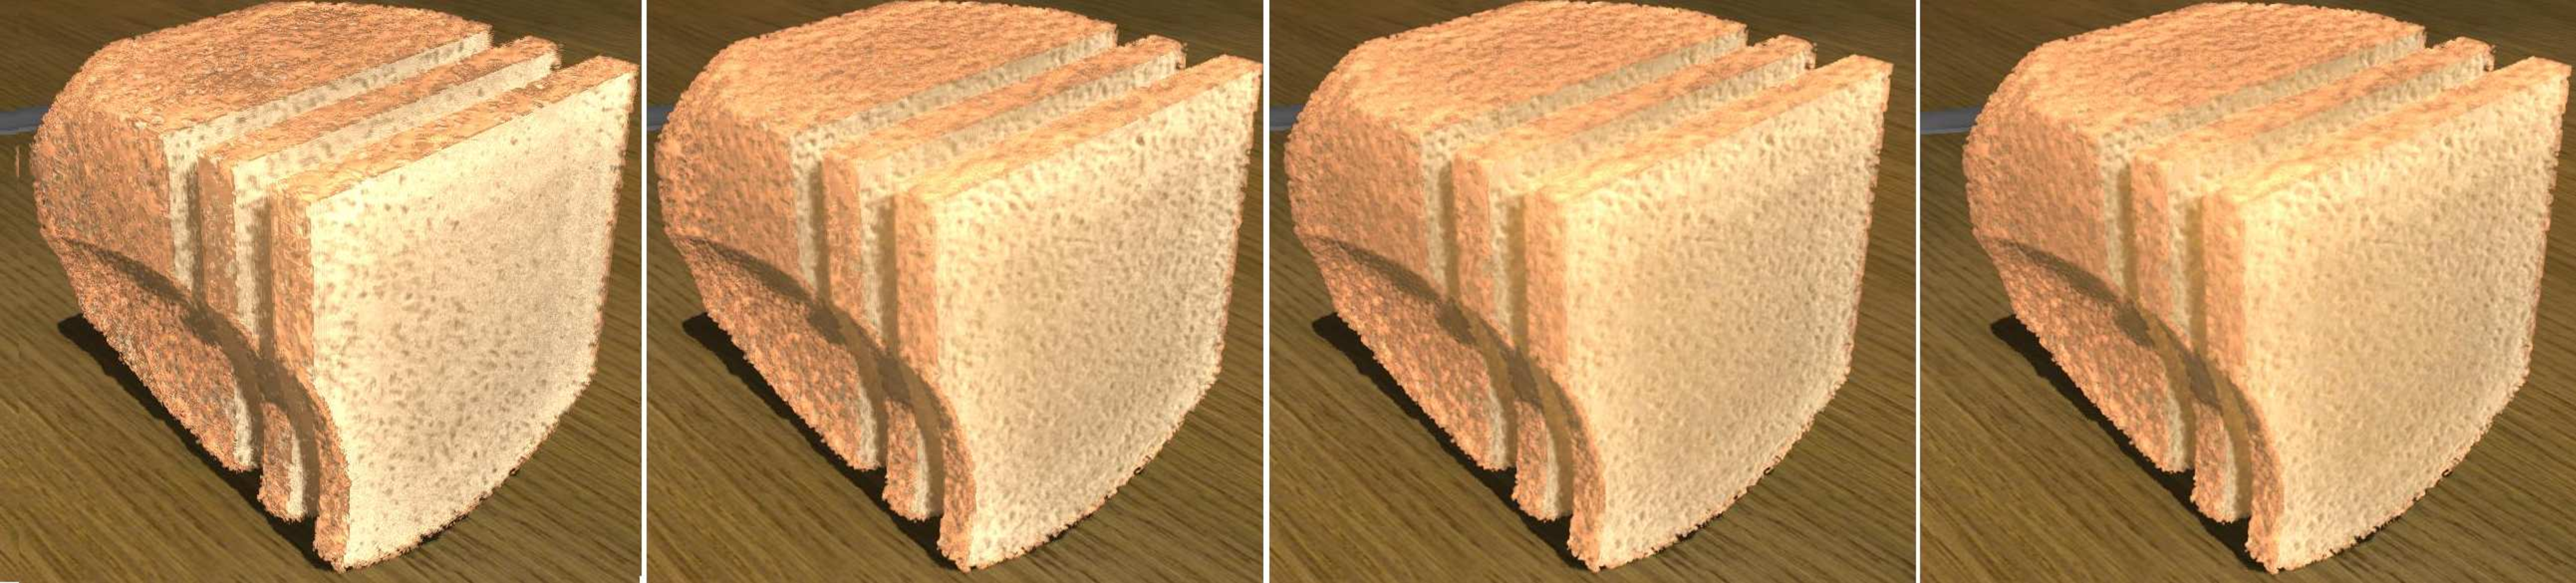
\includegraphics[width=12cm]{stepcount.pdf}

\begin{tabular}{|c|c|c|c|c|c|c|}
\hline
 Pasos del rayo         & 128 &  256 \\
\hline
\hline
 Tiempo total shaders   & 10 ms &  32.5 ms \\
\hline
 Rayo Principal         & 2 ms  & 5 ms  \\
\hline
 Rayos Secundarios      &  8 ms & 27.5 ms  \\
\hline
\end{tabular}
\caption{Detalle de tiempos de renderizado en milisegundos.}
\label{tab:n2}
\end{table}


\end{frame}

%\begin{frame}{Renderizado utilizando más de una escala}
%A la hora de obtener complejidad en la imagen resultante, existen limitaciones en la resolución de la textura.

%Una solución consiste en utilizar más de una textura

%\centerline{\includegraphics[width=10cm]{../figures/multiscale}}

%Textura A muestreada en $(x,y,z)$

%Textura B muestreada en $N\times (x,y,z), N \in \mathbb{R}$

%\end{frame}



\begin{frame}{Conclusiones}
\begin{itemize}
\item Imágenes realistas
\item Tiempo real
\item Implementación simple en GPU
\end{itemize}

\begin{block}{Trabajos a Futuro}
\begin{itemize}
\item Otros materiales
\item Pre-cómputo de la radiancia
\end{itemize}
\end{block}
\end{frame}

\section{Validación}



\begin{frame}
\begin{block}{}
\begin{center}
\vspace{1cm}
\huge{Validación}
\vspace{1cm}
\end{center}
\end{block}
\end{frame}


\subsection{Validación tradicional y automática}
\begin{frame}{Validación tradicional}
\begin{itemize}
\item Se utilizan procesos físicos en el renderizado o modelado
\item Las imágenes pueden pasar una inspección poco detallista sobre su autenticidad
\item Reviewer \#N dice \it{los resultados se ven muy atractivos}
\end{itemize}

En computación gráfica, el camino tradicional es el expuesto.

Proponemos además, validar semi-automáticamente geometrías utilizando fractales.

\end{frame}

\begin{frame}{Validación automática}

Ley fractal $\rightarrow$ geometrías de migas de pan.

\textbf{Espectro Multifractal}

\begin{itemize}
\item Captura distintas estructuras fractales dentro del mismo objeto,
\item o distintos comportamientos fractales dependiendo de la escala.
\end{itemize}

\begin{algorithm}[H]
\begin{algorithmic}[1]
\STATE Obtener espectro multifractal de muestras reales
\FOR{valores de parámetros}
\STATE parámetros $\rightarrow$ muestra sintética $\rightarrow$ espectro
\STATE Comparar espectros reales con sintéticos
\ENDFOR
\STATE Devolver los parámetros más cercanos a los reales
\end{algorithmic}
\end{algorithm}
\end{frame}

%\subsection{Fractales y Multifractales}

\subsection{Multifractales}

%\begin{frame}{Dimensión Box}

%\begin{wrapfigure}{r}{0.5\textwidth}
%\includegraphics[width=6cm]{../figures/fitbox}
%\end{wrapfigure}

%Dada una imagen, se la subdividide en una grilla de dimensiones $M\times M$ donde el largo del lado de cada cuadrado formado es $\delta$. Si $N(\delta)$ representa el n\'umero de cuadrados que contienen al menos un p\'ixel resultado de una binarizaci\'on de la imagen (p\'ixel blanco) para ese $\delta$, la dimensi\'on Box $D_{b}$ queda definida como:\\

%$$D_{b} = \displaystyle\lim_{\delta \to 0}{\frac{\log(N(\delta))}{\log (1/\delta)}}$$


%\end{frame}

%\begin{frame}
%Esto sugiere que podría ser útil utilizar más de una DF para caracterizar los resultados.

%Dimensión generalizada de orden $q$ (método Sandbox):

% \begin{align*}
%D_{q\ne 1}^{sb} &= \frac{1}{q-1} \lim_{R \rightarrow 0}{
%\frac{ln   { \left\langle  (M(R)/M_{0})^{q-1} \right\rangle   }}
%{ln {(R/L)}       }},\\
%D_{q=1}^{sb} &= \lim_{R \rightarrow 0}{
%\frac{ \left\langle ln   { (M(R)/M_{0})  }  \right\rangle}
%{ln {(R/L)}       }},
%\end{align*}

%\noindent donde $M_{0}$ es la cantidad de píxeles blancos en la imagen binarizada y $M(R)$ es el número de puntos que pertenecen a la estructura en un círculo de radio $R$ centrado en un punto de la misma.
%\end{frame}

\begin{frame}
Espectro multifractal en muestras reales ({\em baguette} y pan casero)

Medianas de cada dimensión, con $q \in [-10,10]$.

Comparación con resultados sintéticos, por medio de la \textbf{métrica de error}:

\begin{equation*}
Error = \displaystyle \sum abs(medianas_{real}-medianas_{sint\acute{e}tico}).
\end{equation*}

Las imágenes sintéticas fueron generadas utilizando diversos parámetros en el leudado:

\begin{align*}
N &= \frac{k}{r^{d}},\\ r &= r_{min}+paso*j, j \in [0,\frac{r_{max}}{paso}],
\end{align*}
\noindent $k,d,r_{min},r_{max}$ y $step$ que controlan la generación de burbujas.

\end{frame}

\begin{frame}
\includegraphics[width=4cm]{../figures/bestboxplot}
\includegraphics[width=4.5cm]{../figures/realbin}
\includegraphics[width=2cm]{../figures/best}

\includegraphics[width=4cm]{../figures/bestboxplot2}
\includegraphics[width=4cm]{../figures/realbin2}
\includegraphics[width=2.5cm]{../figures/best2}
\end{frame}



\begin{frame}{Conclusiones}
\begin{block}{}
\begin{itemize}
\item Algoritmo semi-automático para comparar muestras reales y sintéticas
\item Es posible utilizarlo para alimentar la generación a partir de una muestra real, y obtener un pan sintético con características estadísticamente similares.
\item Es posible mejorar el algoritmo hallando automáticamente los parámetros iniciales.
\end{itemize}
\end{block}

\end{frame}

\subsection{Extras}

\begin{frame}
\begin{block}{}
\begin{center}
\vspace{1cm}
\huge{Extras}
\vspace{1cm}
\end{center}
\end{block}
\end{frame}

\begin{frame}{Clasificación de Imágenes de cortes de Pan}
Adicionalmente se estudió el espectro multifractal para \textbf{caracterizar y clasificar} imágenes de cortes reales de pan.

\vspace{0.3cm}

Esto es útil para definir parámetros de calidad que deben respetar los panes reales, y proveer una clasificación automática de los mismos.

\vspace{0.3cm}

Se encontró que el MFS \textbf{clasifica} muestras de panes de manera \textbf{comparable al estado del arte}.

\end{frame}

\begin{frame}
\begin{table}[h!]
\center
% For LaTeX tables use
\begin{tabular}{lllllll}
\hline\noalign{\smallskip}
Método & Haralick & Lbp & SIFT & MFS & MFS CIELab\\ % & Zernicke
\noalign{\smallskip}\hline\noalign{\smallskip}
SVM & 94\% & 78.5\% & 96.5\% & 94.5\% & \textbf{97.5\%} \\
RF  & 91\% & 71.5\% & 92\% & 93.5\% & \textbf{96\%} \\
NN & 79\% & 70\% & 86\%  & 90.5\% & \textbf{92\%} \\
\noalign{\smallskip}\hline
\#FDs & 13 & 36 & 128 & 20 & 60\\
\hline
\end{tabular}
\caption{Resultados de la clasificación de migas de pan para diferentes características del estado del arte y diferentes algoritmos de clasificación.}
\label{tab:other} 
\end{table}
\end{frame}

\begin{frame}
Correlación entre las dimensiones del MFS y \\

\vspace{1cm}

\begin{tabular}{cc}
la fracción de vacío (VF) & el área media de las burbujas (MCA). \\
\includegraphics[width=5cm]{../figures/VF} & \includegraphics[width=5cm]{../figures/MCA} \\
\end{tabular}

\end{frame}

\begin{frame}
Correlación entre las dimensiones del MFS y el desvío estándar del área media de las burbujas (stCA)

\centerline{\includegraphics[width=5cm]{../figures/stMCA}}

%\end{frame}

%\begin{frame}{Conclusiones}

Conclusiones
\begin{itemize}
\item Es posible utilizar el MFS no sólo para clasificar, sino para caracterizar muestras de panes.
\item Clasificación comparable al estado del arte.
\end{itemize}
\end{frame}


\begin{frame}{Validación utilizando Técnicas de Aprendizaje Profundo}



%\end{frame}

%\begin{frame}{Validación utilizando Técnicas de Aprendizaje Profundo}
\centering
\includegraphics[width=3cm]{../figures/deep1}
\includegraphics[width=3cm]{../figures/deep4}

\includegraphics[width=3cm]{../figures/deep2}
\includegraphics[width=3cm]{../figures/deep3}


\vspace{0.4cm}
\url{http://deeplearning.cs.toronto.edu/}

\end{frame}



\section[Conclusiones]{Conclusiones y Trabajos a Futuro}


\begin{frame}
\begin{block}{}
\begin{center}
\vspace{1cm}
\huge{Conclusiones}
\vspace{1cm}
\end{center}
\end{block}
\end{frame}

\subsection{Conclusiones}
\begin{frame}{Conclusiones}
\begin{block}{}
\begin{itemize}
\item Se introdujo un \textbf{algoritmo procedimental} de generación de geometrías \textbf{porosas}.
\item Se presentó un algoritmo \textbf{basado} en el \textbf{proceso real de formación del pan}, eliminando decisiones ad-hoc en la generación de este material, obteniendo estructuras a lo largo de todo el \textbf{proceso de formación}.
\item Se aplicó un algoritmo de renderizado, basado en la interacción lumínica con una escena, produciendo imágenes foto-realísticas de materiales porosos/cocidos/comestibles como pan, esponjas, y piedras. Se obtuvieron imágenes \textbf{foto-realísticas en tiempo real}, por medio de la utilización de la \textbf{GPU}.
\end{itemize}
\end{block}
\end{frame}

\begin{frame}{Conclusiones}
\begin{block}{}
\begin{itemize}
\item Se \textbf{validaron} las geometrías generadas por el proceso inspirado en la formación del pan con muestras reales de pan.
\item Se presentó un método para \textbf{clasificar} muestras de pan, superando a clasificadores del estado del arte.
\end{itemize}
\end{block}
%\end{frame}

%\subsection{Trabajos a futuro}

%\begin{frame}{Trabajos a futuro}
\begin{block}{Trabajos a Futuro}
\begin{itemize}
\item Generación procedimental de huesos y \textbf{otros materiales}
\item Validación tridimensional de los resultados
\item Validación utilizando técnicas de aprendizaje profundo
\item Implementación en \textbf{GPU} de la \textbf{generación procedimental}
\end{itemize}
\end{block}
\end{frame}

\begin{frame}
\centering

?`Preguntas?

\end{frame}

\begin{frame}
\centering

!`Gracias!

\end{frame}
\end{document}
